%%%%%%%%%%%%%%%%%%%%%%%%%%%%%%%%%%%%%%%%%%%%%%%%%%%%%%%%%%%%%%%%%%%%%%%%%%%%%%%
%                       CARREGA DE LA CLASSE DE DOCUMENT                      %
%                                                                             %
% Les opcions admissibles son:                                                %
%      12pt / 11pt            (cos dels tipus de lletra; no feu servir 10pt)  %
%                                                                             %
% catalan/spanish/english     (llengua principal del treball)                 %
%                                                                             %
% french/italian/german...    (si necessiteu fer servir alguna altra llengua) %
%                                                                             %
% listoffigures               (El document inclou un Index de figures)        %
% listoftables                (El document inclou un Index de taules)         %
% listofquadres               (El document inclou un Index de quadres)        %
% listofalgorithms            (El document inclou un Index d'algorismes)      %
%                                                                             %
%%%%%%%%%%%%%%%%%%%%%%%%%%%%%%%%%%%%%%%%%%%%%%%%%%%%%%%%%%%%%%%%%%%%%%%%%%%%%%%

\newcommand{\relativepath}{"style"}
\documentclass[11pt,spanish,listoffigures,listoftables]{\relativepath/tfgetsinf}

%%%%%%%%%%%%%%%%%%%%%%%%%%%%%%%%%%%%%%%%%%%%%%%%%%%%%%%%%%%%%%%%%%%%%%%%%%%%%%%
%                     CODIFICACIO DEL FITXER FONT                             %
%                                                                             %
%    windows fa servir normalment 'ansinew'                                   %
%    amb linux es possible que siga 'latin1' o 'latin9'                       %
%    Pero el mes recomanable es fer servir utf8 (unicode 8)                   %
%                                          (si el vostre editor ho permet)    %
%%%%%%%%%%%%%%%%%%%%%%%%%%%%%%%%%%%%%%%%%%%%%%%%%%%%%%%%%%%%%%%%%%%%%%%%%%%%%%%

\usepackage[utf8]{inputenc}

%%%%%%%%%%%%%%%%%%%%%%%%%%%%%%%%%%%%%%%%%%%%%%%%%%%%%%%%%%%%%%%%%%%%%%%%%%%%%%%
%                        ALTRES PAQUETS I DEFINICIONS                         %
%                                                                             %
% Carregueu aci els paquets que necessiteu i declareu les comandes i entorns  %
%                                          (aquesta seccio pot ser buida)     %
%%%%%%%%%%%%%%%%%%%%%%%%%%%%%%%%%%%%%%%%%%%%%%%%%%%%%%%%%%%%%%%%%%%%%%%%%%%%%%%

\usepackage{graphicx}
\usepackage{wrapfig}

%%%%%%%%%%%%%%%%%%%%%%%%%%%%%%%%%%%%%%%%%%%%%%%%%%%%%%%%%%%%%%%%%%%%%%%%%%%%%%%
%                        DADES DEL TREBALL                                    %
%                                                                             %
% titol, alumne, tutor i curs academic                                        %
%%%%%%%%%%%%%%%%%%%%%%%%%%%%%%%%%%%%%%%%%%%%%%%%%%%%%%%%%%%%%%%%%%%%%%%%%%%%%%%

\title{Refactorización de una infraestructura de bucles MAPE-K como microservicios}
\author{Adriano Vega Llobell}
\tutor{Joan Josep Fons Cors}
\curs{2021-2022}

%%%%%%%%%%%%%%%%%%%%%%%%%%%%%%%%%%%%%%%%%%%%%%%%%%%%%%%%%%%%%%%%%%%%%%%%%%%%%%%
%                     PARAULES CLAU/PALABRAS CLAVE/KEY WORDS                  %
%                                                                             %
% Independentment de la llengua del treball, s'hi han d'incloure              %
% les paraules clau i el resum en els tres idiomes                            %
%%%%%%%%%%%%%%%%%%%%%%%%%%%%%%%%%%%%%%%%%%%%%%%%%%%%%%%%%%%%%%%%%%%%%%%%%%%%%%%

\keywords{????, ?????????, ????, ?????????????????} % Paraules clau
         {?????, ???, ???????????????}              % Palabras clave
         {?????, ????? ?????, ?????????????}        % Key words

%%%%%%%%%%%%%%%%%%%%%%%%%%%%%%%%%%%%%%%%%%%%%%%%%%%%%%%%%%%%%%%%%%%%%%%%%%%%%%%
%                              INICI DEL DOCUMENT                             %
%%%%%%%%%%%%%%%%%%%%%%%%%%%%%%%%%%%%%%%%%%%%%%%%%%%%%%%%%%%%%%%%%%%%%%%%%%%%%%%
\begin{document}

\bibliographystyle{ieeetr}

%%%%%%%%%%%%%%%%%%%%%%%%%%%%%%%%%%%%%%%%%%%%%%%%%%%%%%%%%%%%%%%%%%%%%%%%%%%%%%%
%              RESUMS DEL TFG EN VALENCIA, CASTELLA I ANGLES                  %
%%%%%%%%%%%%%%%%%%%%%%%%%%%%%%%%%%%%%%%%%%%%%%%%%%%%%%%%%%%%%%%%%%%%%%%%%%%%%%%

\begin{abstract}
????
\end{abstract}
\begin{abstract}[spanish]
????
\end{abstract}
\begin{abstract}[english]
????
\end{abstract}

%%%%%%%%%%%%%%%%%%%%%%%%%%%%%%%%%%%%%%%%%%%%%%%%%%%%%%%%%%%%%%%%%%%%%%%%%%%%%%%
%                              CONTINGUT DEL TREBALL                          %
%%%%%%%%%%%%%%%%%%%%%%%%%%%%%%%%%%%%%%%%%%%%%%%%%%%%%%%%%%%%%%%%%%%%%%%%%%%%%%%

\mainmatter

%%%%%%%%%%%%%%%%%%%%%%%%%%%%%%%%%%%%%%%%%%%%%%%%%%%%%%%%%%%%%%%%%%%%%%%%%%%%%%%
%                         CAPITOLS (tants com calga)                          %
%%%%%%%%%%%%%%%%%%%%%%%%%%%%%%%%%%%%%%%%%%%%%%%%%%%%%%%%%%%%%%%%%%%%%%%%%%%%%%%

%%%%%%%%%%%%%%%%%%%%%%%%%%%%%%%%%%%%%%%%%%%%%%%%%%%%%%%%%%%%%%%%%%%%%%%%%%%%%%%
%                                  INTRODUCCIO                                %
%%%%%%%%%%%%%%%%%%%%%%%%%%%%%%%%%%%%%%%%%%%%%%%%%%%%%%%%%%%%%%%%%%%%%%%%%%%%%%%

\chapter{Introducción}
\label{chap:introduccion}

La revolución digital\footnote{\url{https://es.wikipedia.org/wiki/Revoluci\%C3\%B3n_Digital}} ha permeado en todos los aspectos de nuestras vidas. En nuestro día a día usamos una gran variedad de aplicaciones informáticas: redes sociales, ofimática, comercios electrónicos\dots Muchas de ellas se encuentran alojadas en la red, en servidores externos.

Para las aplicaciones web, uno de sus requisitos claves es la \textbf{disponibilidad}. \cite{birmanAddingHighAvailability2004} Nuestros servicios deben estar en funcionamiento en todo momento para atender a nuestros usuarios. Tomemos por ejemplo el caso de una tienda \foreign{english}{on-line}. La plataforma debe estar disponible el mayor tiempo posible. Si surgiera una incidencia y se degrada la capacidad de atender a clientes, o directamente no podemos atender a ninguno, perderemos ingresos.

Para atender estas incidencias, no es efectivo depender de operarios humanos. \cite{ibmcorporationArchitecturalBlueprintAutonomic2006} Es muy costoso tener a alguien pendiente de la aplicación las veinticuatro horas del día para atender las incidencias. Sería preferible que nuestro sistema sea capaz de \textbf{adaptarse automáticamente} a las distintas situaciones que surjan durante su operación. Recurrir al operario humano debería ser el último recurso.

En el ámbito de la computación autónoma (\foreign{english}{autonomic computing}) encontramos el concepto de \textbf{sistemas auto-adaptativos}. Son sistemas capaces de ajustar su comportamiento en tiempo de ejecución en base su estado y el del entorno para alcanzar sus objetivos de operación. \cite{ibmcorporationArchitecturalBlueprintAutonomic2006} Esto es posible mediante el uso de \textbf{bucles de control}. \cite{brunEngineeringSelfAdaptiveSystems2009} Gracias a ellos, podremos dotar a los sistemas de capacidades para adaptarse a entornos cambiantes, resolver conflictos operacionales e incluso a la optimizarse dinámicamente.

Siguiendo con el ejemplo de la tienda on-line, un ejemplo de auto-adaptación sería adaptarse a los picos de demanda. Cuando tengamos mayor afluencia de clientes, debe ser capaz de aumentar su capacidad de cómputo. En cambio, cuando la afluencia baje, deberá ser capaz de reducirla.

\section{Motivación}

En este trabajo se quiere explorar el diseño de soluciones auto-adaptativas que estén preparadas para desplegarse en la nube. Para ello se tomó como punto de partida la infraestructura FaDA\footnote{Página oficial: \url{http://fada.tatami.webs.upv.es/}} (desarrollada por el grupo PROS/Tatami\footnote{Página oficial: \url{http://www.pros.webs.upv.es/}} del instituto VRAIN/UPV\footnote{Página oficial: \url{https://vrain.upv.es/}}). Esta propone una estrategia para la ingeniería de sistemas auto-adaptativos usando bucles de control MAPE-K\cite{ibmcorporationArchitecturalBlueprintAutonomic2006, fonsServiciosAdaptivereadyPara2021}.

Actualmente, el bucle de control de FaDA está implementado como un servicio monolítico. Todos sus componentes operan dentro del mismo proceso, incluidos los específicos para sistemas manejados (sondas, monitores\dots). Se trata por tanto de una implementación muy rígida. En caso de querer modificar algún componente, hay que redesplegarlo entero.

Por ello, se buscó \textbf{dividir su funcionalidad en microservicios}. Es decir, cambiar la topología de la solución. Con ello, se lograría independizar los componentes y su despliegue. Además, facilitaría escalar horizontalmente la capacidad del sistema en base a la carga.

\section{Objetivos}

Para el desarrollo del trabajo nos planteamos los siguientes objetivos:

\begin{enumerate}
  \item Rediseñar la arquitectura existente para soluciones auto-adaptativas y prepararla para desplegarse nativamente como microservicios en la nube. Esto implica determinar los componentes en los que dividiremos la funcionalidad del bucle y los mecanismos de comunicación para conectarlos.

  \item Definir directrices para la implementación de los diferentes componentes adaptativos específicos de una solución: monitores, sondas, efectores\dots

  \item Desarrollar un caso práctico para demostrar la viabilidad y aplicabilidad de nuestra propuesta.
\end{enumerate}

\section{Estructura de la memoria}

El trabajo se divide en cuatro grandes secciones. La primera de ellas es el \textbf{marco teórico}. En el capítulo \ref{chap:contexto_tecnologico} se presentan algunos conceptos de la computación autónoma y los bucles de control. Se describirá la arquitectura MAPE-K, en la que se basa el trabajo. También definiremos algunos conceptos de arquitecturas de \foreign{english}{software} que nos serán de interés.

La segunda parte de este trabajo trata sobre la \textbf{migración del sistema existente} a una arquitectura basada en microservicios. Para ello, se introducirá el sistema actual: el bucle MAPE-K \foreign{english}{Lite} de FaDA (capítulo \ref{chap:sistema_original}). A continuación, en el capítulo \ref{chap:diseño} presentamos nuestra propuesta arquitectónica. Se describirá los distintos componentes que la conforman y los mecanismos de comunicación para conectarlos. Finalmente, en el capítulo \ref{chap:implementación}, detallaremos paso a paso nuestra implementación.

La tercera sección del trabajo describe un \textbf{caso de estudio} (capítulo \ref{chap:caso_estudio}). En él, se desarrolla un sistema auto-adaptativo básico de climatización. Nos sirvió para aplicar nuestra arquitectura en la práctica y verificar su funcionamiento. Sirve cómo implementación referencia para otras soluciones autoadaptativas.

Finalmente, cerraremos el trabajo con una descripción del proceso de \textbf{despliegue del sistema y pruebas} (capítulo \ref{chap:despliegue}). Para validar nuestra arquitectura realizamos distintos tipos de pruebas de funcionalidad y rendimiento. En base a los resultados, presentamos cambios que podrían hacerse sobre nuestra propuesta arquitectónica. A continuación, presentamos las conclusiones  generales (capítulo \ref{chap:conclusiones}). Se presentarán también las vertientes por las que se podría continuar ampliando el trabajo en un futuro.

%\section{Notes bibliografiques} %%%%% Opcional

%????? ????????????? ????????????? ????????????? ????????????? ?????????????

\textcolor{red}{Añadir diagrama de Gant con los 7 hitos}


\chapter{Contexto Tecnológico}
\label{chap:contexto_tecnologico}

\section{Computación autónoma y bucles de control}

Según \cite{ibmcorporationArchitecturalBlueprintAutonomic2006}, la \textbf{computación autónoma} tiene como objetivo dotar a los sistemas de \textbf{autonomía} en su operación. Es decir, capacidades para gestionarse a si mismos. Los sistemas deberán adaptarse a los cambios en su entorno de ejecución. Con esto, buscamos alcanzar una reducción en el coste de operación y hacer más manejable la complejidad de los sistemas.

Las adaptaciones pueden ser de distintos tipos: cambios en sus parámetros de configuración, habilitar o deshabilitar funcionalidades, etc. Estas se realizan en base a directivas de alto nivel, los objetivos. Un operario humano define las metas que el sistema debe alcanzar, y este intentará planificar acciones correctivas para alcanzarlo.

Siguiendo con el ejemplo de la tienda \foreign{english}{on-line}, el operario podría definir un umbral máximo de carga por cada instancia. Cuando se supere, el sistema podría decidir que se requiere una acción correctiva. Por ejemplo, esta acción podría consistir en desplegar nuevas instancias del servicio. Cuando la carga de los servicios baje, podrá optar por eliminarlas.

Para implementar estas capacidades de adaptación se recurre a la teoría de control y al \textbf{bucle de control} (o \emph{feedback loop}). \cite{brunEngineeringSelfAdaptiveSystems2009} Se trata de un proceso iterativo para la gestión de sistemas. A partir de información sobre el estado del sistema y su entorno, pauta acciones correctivas. Estas se basan en heurísticas definidas por los administradores del sistema. Puede dividirse en cuatro etapas (figura \ref{fig:bucle-control}):

\begin{figure}[h]
  \centering
  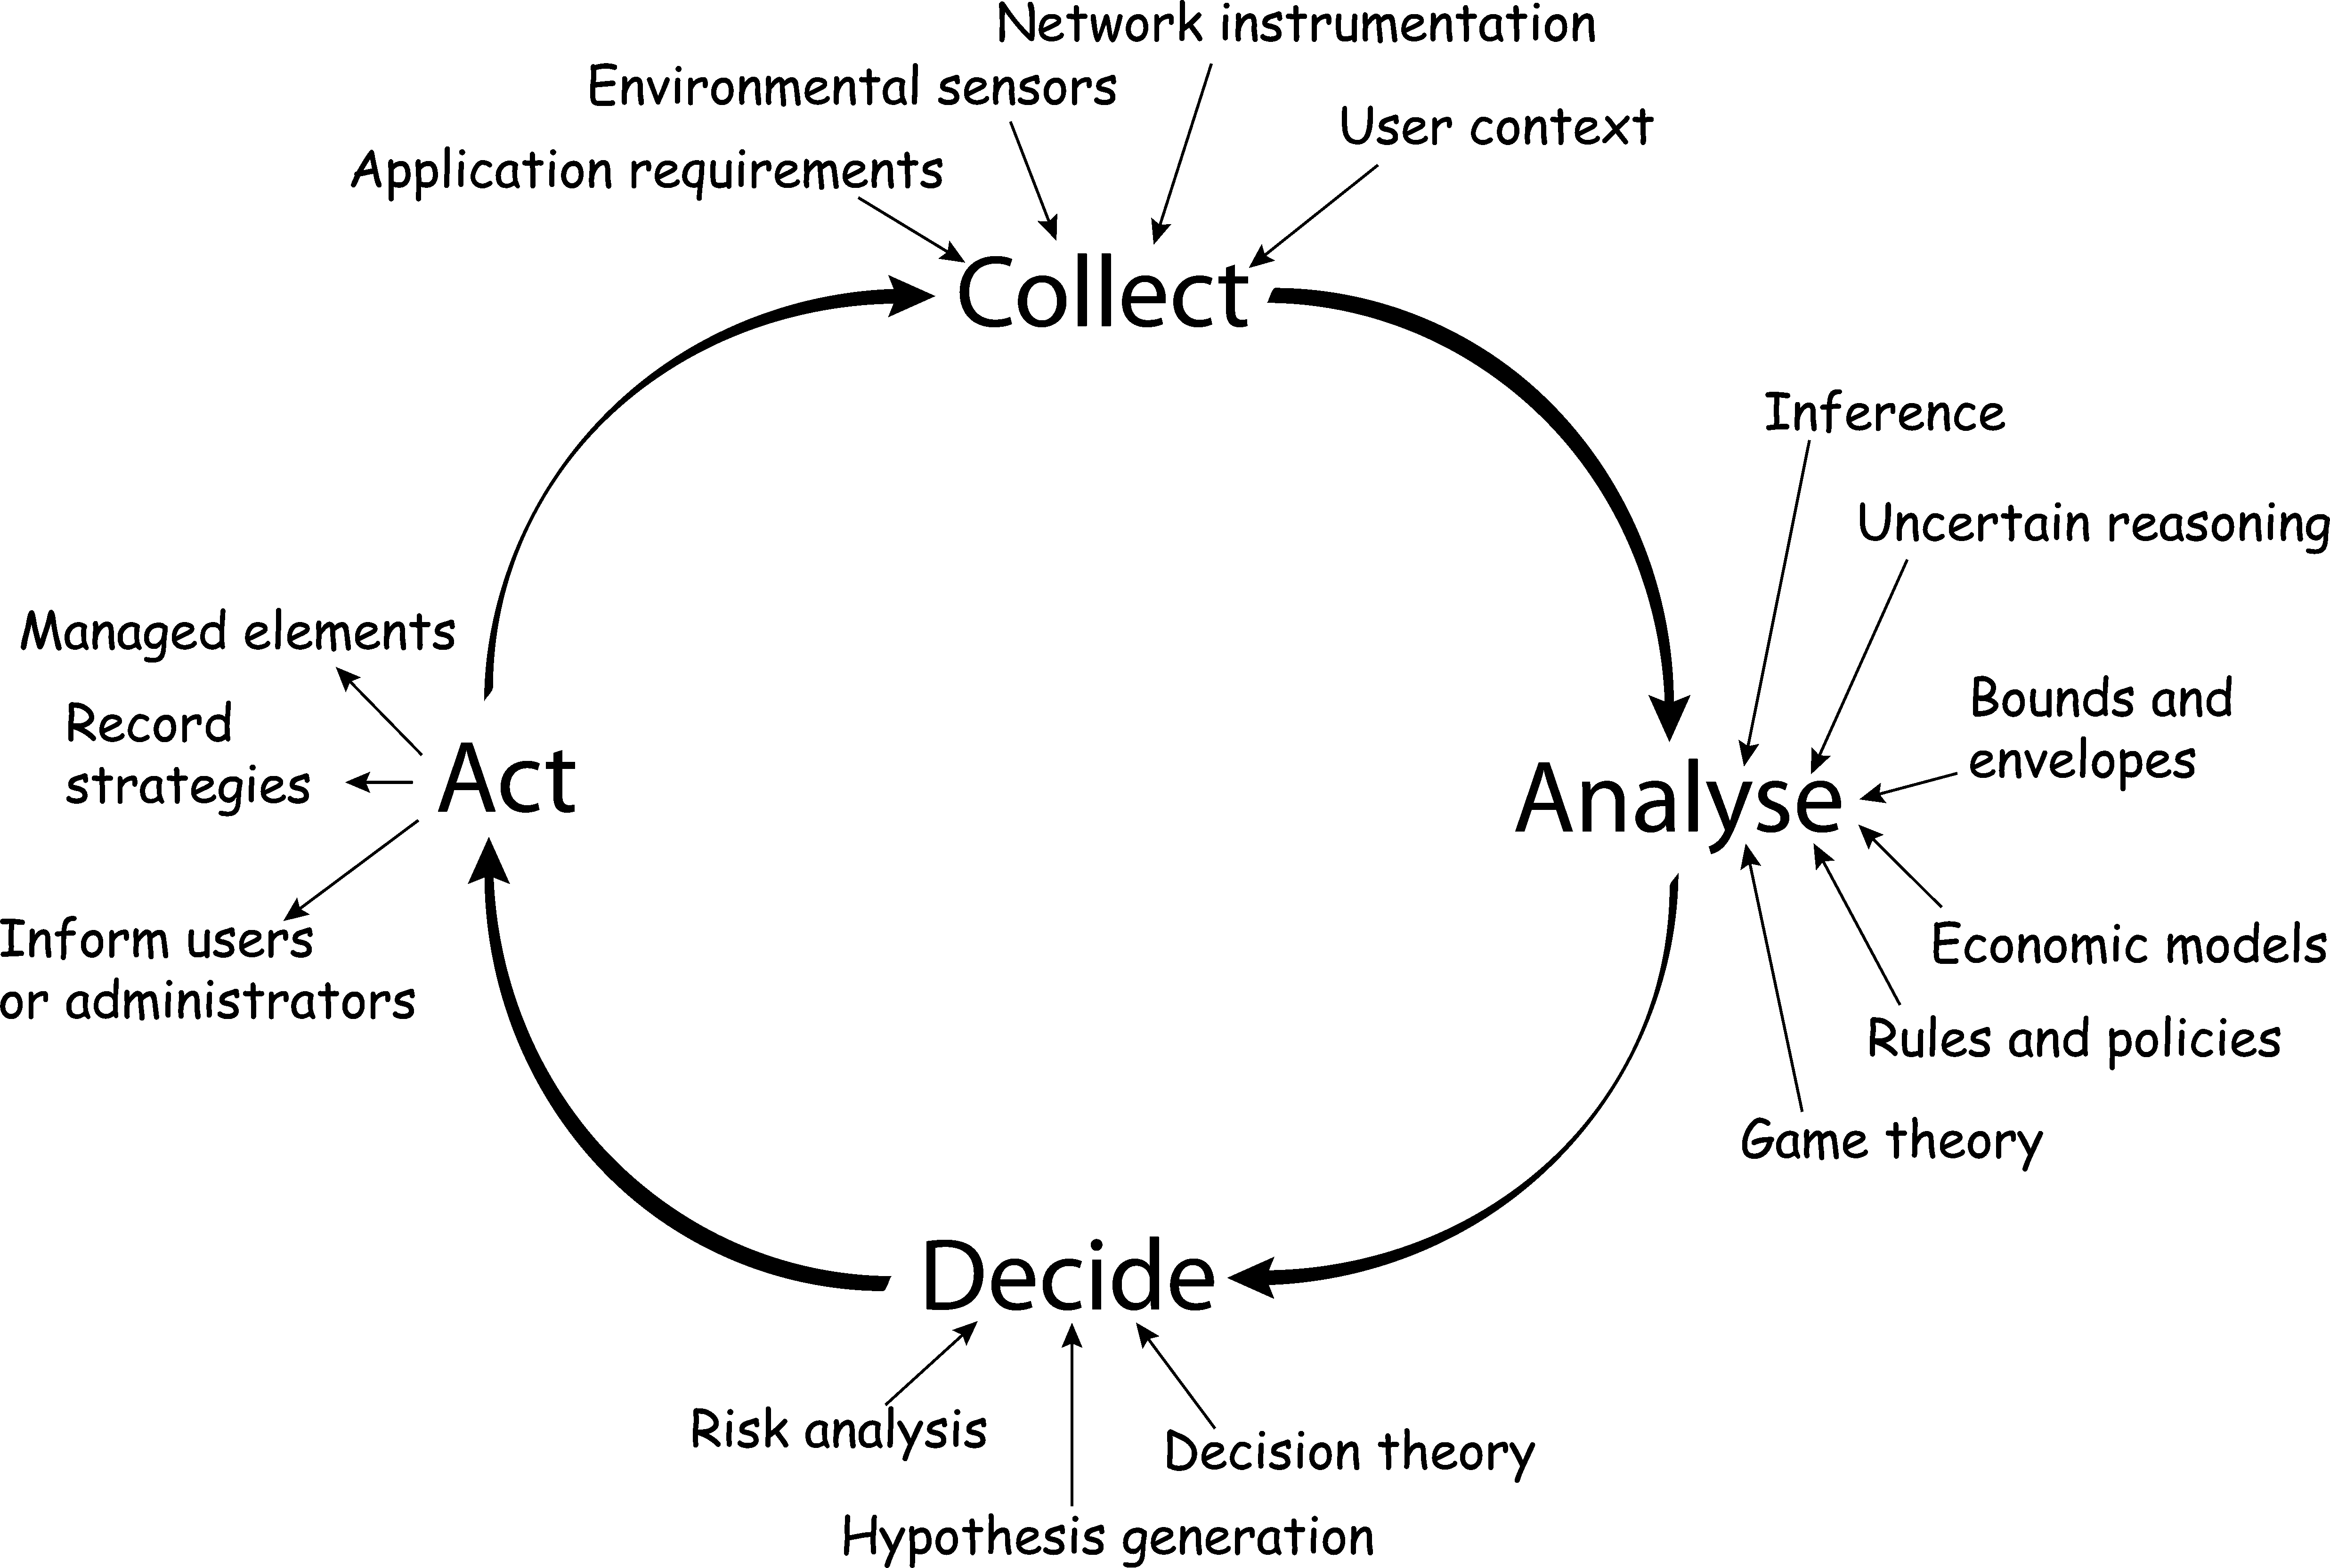
\includegraphics[scale=0.065]{cap_introduccion/images/feedback-loop}
  \caption[Un bucle de control genérico. Consta de cuatro actividades: Recopilar información, analizarla, decidir y actuar si procede.]{Un bucle de control genérico. Consta de cuatro actividades: Recopilar información, analizarla, decidir y actuar si procede. Obtenida de \cite{dobsonSurveyAutonomicCommunications2006}.}
  \label{fig:bucle-control}
\end{figure}

\begin{itemize}
  \item \textbf{Recopilar información}: El bucle \textbf{monitoriza} el estado del sistema a través de \textbf{sondas}. Estas reportan información del sistema y del entorno de ejecución. Pueden ser métricas de rendimiento, estado de los componentes, cambios en en el entorno, etc.

  Estos datos en bruto deben ser limpiados, filtrados y agregados para sintetizarlos en propiedades de nuestro interés. Si se considera que son relevantes, se almacenan para informar las siguientes etapas del bucle.

  \item \textbf{Analizar}: Basándose en la información considerada de interés, la etapa de análisis debe identificar \textbf{síntomas}: indicadores de una situación que requiera de nuestra atención. Puede ser mediante heurísticas predefinidas, análisis estadístico u otros métodos. Un ejemplo de síntoma sería ''uso de CPU elevado'', ''número elevado de mensajes encolados en un sistema de mensajería'', etc.

  \item \textbf{Decidir}: \textcolor{red}{A partir de los síntomas, el bucle debe determinar si es necesario tomar alguna acción. Si detecta que no estamos cumpliendo los objetivos, o que puede mejorarse la configuración actual, .} \textbf{Planifica} qué acciones deben llevarse a cabo para que el sistema se adapte y alcance una configuración deseable. Por ejemplo, si hay muchos mensajes encolados, se podría solicitar el iniciar otra instancia del servicio que los consuma y procese en paralelo.

  \item \textbf{Actuar}: Si se ha planificado alguna acción, se intentará \textbf{ejecutar} en esta etapa final. Mediante \textbf{efectores} en el sistema, el bucle es capaz de modificar su configuración. Dependiendo del éxito de ejecución, la adaptación se lleva a cabo o no. Finalizada esta etapa, se vuelve a recopilar información y arranca de nuevo el proceso.
\end{itemize}


\textcolor{red}{Hablar de human in the loop: solicitamos la intervención del humano cuando no contamos con suficiente información para tomar una acción correctiva.}

Este tipo de proceso está presente en gran variedad de contextos como puede ser operación de plantas industriales, \cite{climentpenadesDissenyPrototipatSolucions2020a}  en procesos naturales, etc. \textcolor{red}{ampliar}

\textcolor{red}{Hablar de agentes autónomos como aplicación práctica. \cite{savaglioAgentbasedInternetThings2020}}

En la ingeniería de \emph{software}, encontramos los bucles de control en dos variantes distintas: bucles de control implícitos o explícitos. La más habitual es la primera: se encuentran implícitos en la implementación de los procesos del sistema. \cite{brunEngineeringSelfAdaptiveSystems2009} No son componentes externos dedicados.

Por otro lado, aproximaciones como las de \cite{garlanIncreasingSystemDependability2003} o \cite{ibmcorporationArchitecturalBlueprintAutonomic2006} optan por la segunda: bucles como componentes externos. Esto permite separar la funcionalidad de las capacidades de adaptación.  Al dividirse estas responsabilidades, se puede reducir la complejidad de la implementación. En este trabajo nos centraremos en esta segunda variante.

\section{Arquitecturas para sistemas autónomos: Bucles MAPE-K}
\label{sec:bucles-mapek}

%% TODO: Buscar sinonimos de sistema..

Un estilo arquitectónico muy representativo es el basado en bucles MAPE-K \cite{ibmcorporationArchitecturalBlueprintAutonomic2006, fonsServiciosAdaptivereadyPara2021} propuesto por IBM. Se trata de una referencia arquitectónica para desarrollar sistemas distribuidos autónomos. Nace con el objetivo hacer más manejable la complejidad de estos sistemas; y reducir sus costes de operación, requiriendo de la minima intervención humana.

Su componentes principales son los \textbf{elementos autónomos}. Cada uno de estos es capaz de autogestionarse, y colaborar en conjunto con el resto de elementos autónomos del sistema  para alcanzar los objetivos. \textcolor{red}{¿Agent based?} A su vez, estos pueden dividirse en dos partes: los recursos manejados y un manejador autónomo (el bucle de control).

Los \textbf{recursos manejados} son las unidades de funcionalidad. Puede ser cualquier tipo de recurso, \emph{hardware} o \emph{software}. Para dotarlos de capacidad de autoadaptación, los emparejamos con un \textbf{manejador autónomo}: el bucle de control. Gestiona al recurso en base a la información que recoge del entorno de ejecución y las políticas que guían su adaptación.

El bucle es de tipo externo, ya que es un componente distinto al que implementa la funcionalidad. Por tanto, el recurso debe implementar puntos de contacto (\textbf{\emph{touchpoints}}): interfaces que permitan obtener información de su estado (sondas) y cambiar su configuración (efectores).

Estos elementos autónomos se auto-gestionan en base a \textbf{políticas}: un conjunto de objetivos de alto nivel definidos por sus administradores. El sistema tratará de mantener su cumplimiento durante su ejecución. Para alcanzarlos, el manejador autónomo planifica cambios en la configuración del recurso manejado.

\subsection{Estructura del bucle MAPE-K}

En la figura \ref{fig:autonomic-element} mostramos una representación de un elemento autónomo. Distinguimos las dos partes principales: el manejador y el recurso. El manejador contacta con el recurso a través de sus sensores y efectores. Podemos apreciar los componentes que conforman el bucle, y que describimos a continuación: \cite{ibmcorporationArchitecturalBlueprintAutonomic2006}

\begin{figure}[h]
  \centering
  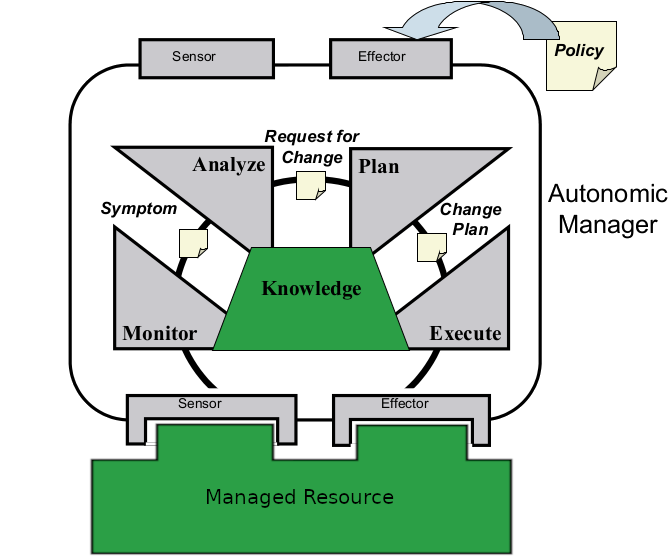
\includegraphics[scale=2]{cap_contexto_tecnologico/images/autonomic-element}
  \caption[Representación de un elemento autónomo. Distinguimos el recurso manejado y el manejador autónomo. El manejador es un bucle MAPE-K (\emph{Monitor}, \emph{Analysis}, \emph{Planification}, \emph{Execution} y \emph{Knowledge})]{Representación de un elemento autónomo. Distinguimos el recurso manejado y el manejador autónomo. El manejador es un bucle MAPE-K. Basada en imagen de \cite{ibmcorporationArchitecturalBlueprintAutonomic2006}.}
  \label{fig:autonomic-element}
\end{figure}

Para presentar estos componentes, describiremos un ejemplo de cómo se manejaría un servicio web. Nos centraremos en escalar este servicio en base a la carga del sistema. Deseamos que, en caso de carga elevada, se desplieguen nuevas instancias. Si la carga bajara, el sistema debería eliminar las instancias redundantes.

\subsubsection{Sondas}

Para monitorizar el recurso y su entorno debemos \textbf{instrumentarlos}. Consiste en implementar \textbf{sondas} que expongan datos relevantes a los monitores del bucle. Pueden capturar y transmitir cualquier aspecto que queramos controlar: \emph{health checks}, rendimiento del servicio u otras propiedades del sistema.

Para nuestro servicio web, una métrica relevante sería el número de peticiones por segundo que está atendiendo. La sonda reportaría el número de peticiones que se han atendido hasta un determinado momento.

\subsubsection{Monitor}

El monitor recibe las mediciones de las sondas. Se encarga de recogerlas, agregarlas y filtrarlas para extraer información relevante. La información se almacenará como propiedades de adaptación en la base de conocimiento.\cite{fonsEspecificacionSistemasAutoadaptativos2021} El monitor y las sondas componen la etapa de recopilar información de los bucles de control.

Siguiendo con nuestro ejemplo, el monitor recibiría el número de peticiones atendidas, y las agregaría en una métrica de serie temporal de peticiones por segundo. Esta sería una de nuestras propiedades de adaptación. En base a ella, las siguientes etapas tomarán las decisiones convenientes para escalar nuestro servicio.

\subsubsection{Base de conocimiento}

La base de conocimiento (\emph{knowledge base}) es el componente base de toda la arquitectura. Informa a todas las etapas del bucle de control. Por lo que se trata de un componente transversal. \textcolor{red}{Es una arquitectura knowledge-driven \cite{taylorSoftwareArchitectureFoundations2009}.}

Está compuesta por una o más fuentes de información que el bucle tiene a su disposición. A partir de ellas, se almacenan las \textbf{propiedades de adaptación}. Estas describen el estado pasado y presente del sistema y su entorno: métricas, componentes, conexiones entre ellos, parámetros de configuración\dots

En conjunto, estas propiedades conforman un modelo abstracto del estado del recurso manejado que se mantiene en tiempo de ejecución. \cite{garlanIncreasingSystemDependability2003}. Las demás etapas del bucle operan en base a él. Como veremos más adelante, los efectores se encargan de traducir las acciones correctivas del modelo de alto nivel a términos del recurso manejado.

\subsubsection{Analizador}

En base al modelo abstracto del sistema, podemos razonar sobre el estado actual sin acoplarnos al recurso manejado. Podemos definir heurísticas que nos permitan detectar situaciones que requieran de una acción correctiva. Esta es la función del analizador.

Para implementarlo, una posible aproximación es mediante \textbf{reglas de adaptación}. Estas pueden dividirse en dos partes: la condición y la acción. La condición se define a partir de las propiedades de adaptación y evalúa si es necesario ejecutar la acción correctiva.

La acción de la regla describe una \textbf{propuesta de cambio} en la configuración del sistema. Estas se formulan en base a \textbf{operadores arquitectónicos}. \cite{garlanIncreasingSystemDependability2003} Dependiendo del estilo arquitectónico de nuestro sistema, tendremos disponibles una serie de operaciones para alterar su arquitectura.

Por ejemplo, nuestro recurso manejado podría estar implementado como microservicios. En este caso, los operadores podrían consistir en desplegar o eliminar servicios, establecer conexiones entre los servicios, eliminarlas, o cambiar las propiedades de configuración del servicio. \cite{fonsServiciosAdaptivereadyPara2021}

Las reglas se suscriben a cambios de las propiedades de las que dependen. Cuando ocurra alguno, se evalúa su condición. Si esta se cumple, se ejecuta la acción asociada. En caso contrario, no hará nada.

Respecto al servicio web, definiremos reglas tomando el valor del número de peticiones por segundo. Podemos definirlas con umbrales para este valor: si es muy alto, la regla solicita el despliegue de una nueva instancia. Cuando la carga baje, y si el servicio está replicado, podremos eliminarlas.

\subsubsection{Planificador}

Si alguna regla se dispara, el planificador recibe su propuesta de cambio. Este módulo se encarga de validar las acciones propuestas y agruparlas en un \textbf{plan de adaptación}. Para ello, recurre al conocimiento y compara el estado actual del sistema con las acciones solicitadas.

Deberá verificar si estas acciones siguen siendo necesarias. Podría ocurrir que desde que se solicitaron hasta que se genera el plan de adaptación, haya cambiado el estado del sistema. También comprobará si es seguro aplicarlas, ya que no deben dejar el sistema en un estado inconsistente.

\subsubsection{Ejecutor}

En la etapa final del bucle tenemos al ejecutor. Recibe el plan de adaptación del planificador y, como su nombre indica, es el encargado de ejecutarlo. Para ello, manipula los efectores del recurso manejado. Deberá identificar a cuáles debe transmitir el comando para realizar la adaptación.

Si una adaptación se lleva a cabo correctamente, deberá reflejarse en el conocimiento el nuevo estado, una vez se confirme. En caso de error, deberemos tener mecanismos de compensación que reviertan las acciones ejecutadas. Así, evitamos que el sistema quede en un estado inconsistente.

\subsubsection{Efectores}

Los \textbf{efectores} son el segundo tipo de \foreign{english}{touchpoint} que debe ofrecer el recurso manejado. Ofrecen una interfaz común que permite al bucle modificar la configuración o estado del sistema. Deberán interpretar estas acciones, descritas en conceptos de alto nivel (nivel de arquitectura) y traducirlas a acciones de más bajo nivel (en términos del propio sistema). \cite{garlanIncreasingSystemDependability2003} Es decir, deberán determinar cómo ejecutarlas en el recurso manejado.

La comunicación entre este servicio y el sistema es un tanto especial: dependerá del sistema manejado; de si tenemos control sobre su implementación. Si no es así, tendremos que adaptarnos a la implementación que ofrezca este (HTTP, mensajería...).

En el caso del servicio web, la acción correspondiente sería desplegar o eliminar instancias. El efector conocerá el sistema de despliegue (p.e. Docker) y cómo solicitar la activación o desactivación de un servicio.

\subsection{Sistemas distribuidos basados en elementos autónomos}

\textcolor{red}{Si nos fijamos en la figura \ref{fig:autonomic-element}, veremos que en la parte superior del elemento autónomo figuran sondas y efectores. Esto nos indica que a su vez, pueden actuar también como recursos manejados. Esto nos permite poner por encima de este otro manejador autónomo que actúe como un \textbf{orquestador}. \cite{ibmcorporationArchitecturalBlueprintAutonomic2006}. Estos gestionan a un nivel superior uno o más elementos autonómicos. Son por tanto, elementos componibles.}

\textcolor{red}{Este orquestador podría estar responsabilizado de otras tareas de más alto nivel.}

\textcolor{red}{Por encima de estos orquestadores, finalmente, tendríamos al administrador u operario humano.}
\textcolor{red}{Hablar del \emph{human manager}, la capa superior al sistema. Emite las políticas y monitoriza su funcionamiento a través de las sondas del bucle orquestador.}


\textcolor{red}{¿Hablar del nivel en el que se encuentra el bucle de control? Sistema, infraestructura, mixto, mesh \cite{mendoncaGeneralityVsReusability2018}}


\chapter{Arquitectura de la solución}

En este capítulo vamos a describir la arquitectura que hemos diseñado para distribuir el bucle MAPE-K. Partimos de un sistema con una \textcolor{red}{división funcional ya definida}, por lo que será sencillo delimitar los componentes. El foco de este capítulo serán entonces los \textbf{conectores de \emph{software}}. Necesitamos establecer qué estrategias de comunicación utilizaremos para comunicar los componentes.

Comenzaremos dando una breve introducción a las arquitecturas de \emph{software} y los elementos que las componen. Después, describiremos la arquitectura de nuestra solución y el proceso que hemos seguido para llegar hasta ella.

\section{Arquitecturas de \emph{software}}

Según \cite{taylorSoftwareArchitectureFoundations2009}, la \textbf{arquitectura de un sistema \emph{software}} es el conjunto de todas las \textbf{decisiones principales de diseño} que se toman durante su ciclo de vida; aquellas que sientan las bases del sistema. Estas afectan a todos sus apartados: la funcionalidad que debe ofrecer, la tecnología para su implementación, cómo se desplegará, etc. En conjunto, definen una pauta que guía (y a la vez refleja) el diseño, la implementación, la operación y la evolución del sistema.

Todos los sistemas \emph{software} cuentan con una. La diferencia radica en si esta ha sido diseñada y descrita explícitamente o ha quedado implícita en su implementación. \cite{taylorSoftwareArchitectureFoundations2009} En el segundo caso es probable que, con el paso del tiempo, se ``erosione`` su arquitectura: se implementan funcionalidades sin respetar la estructura. También se olvida el por qué de ciertas decisiones. En general, se vuelve más difícil de mantener. Se convierte en una ''gran bola de barro''. \cite{footeBigBallMud1997}

Por tanto, es vital dedicar tiempo para definirla atendiendo a las necesidades de nuestro sistema. Una buena arquitectura es capaz dotar de estructura a nuestro sistema. \cite{martinCleanArchitectureCraftsman2018} Mientras se respete la arquitectura, y se mantenga actualizada, esta estructura. Una buena arquitectura nos ofrece una serie de ventajas, como facilitar su desarrollo, mayor extensibilidad.

\subsection{Componentes de una arquitectura}

Otra posible definición de arquitectura la encontramos en el estándar IEEE 42010-2011 \cite{ieeeStandard420102011Systems2011}: es "\emph{un conjunto de conceptos o propiedades fundamentales, personificados por sus elementos, sus relaciones, y los principios que guían su diseño y evolución}".

Podemos describirlas entonces usando tres conceptos: \cite{perryFoundationsStudySoftware1992}

    \begin{itemize}
        \item \textbf{Componentes} (o elementos): Son las piezas fundamentales que conforman el sistema. Representan las unidades de funcionalidad de la aplicación. Se utilizan para describir \textbf{\emph{qué}} partes componen el sistema. Por ejemplo: un módulo, un servicio web...

        \item \textbf{Forma}: El conjunto de propiedades y relaciones de un elemenento con otros o con el entorno de operación. Describe \textbf{\emph{cómo}} está organizado el sistema. Por ejemplo: un servicio A contacta con otro, B, usando una llamada HTTP.

        \item \textbf{Justificación}: Razonamiento o motivación de las decisiones que se han tomado. Responden al \textbf{\emph{por qué}} algo se hace de una manera determinada. Normalmente no pueden deducirse a partir de los elementos y la forma, por lo que es necesario describirlos explícitamente.

    \end{itemize}

\subsubsection{Elementos}

El primer tipo de elemento que debemos tratar son los componentes. Según \cite{taylorSoftwareArchitectureFoundations2009}, los \textbf{componentes} son ``elementos arquitectónicos que encapsulan un subconjunto de la funcionalidad y/o de los datos del sistema``.
Dependiendo de las características de nuestro sistema (y del nivel de abstracción que usemos) pueden tomar distintas formas: objetos, módulos dentro un mismo proceso, servicios distribuidos, etc.

\begin{wrapfigure}{r}{0.40\linewidth}
  \centering
  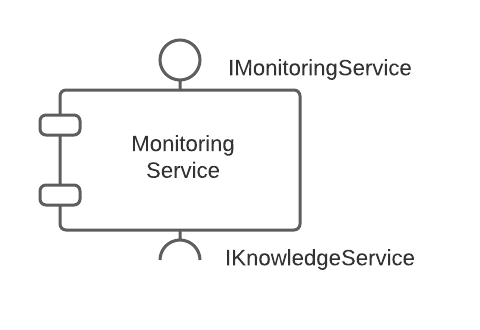
\includegraphics[scale=0.8]{cap_arquitectura/images/componente-ejemplo}
  \caption{El servicio de monitorización representado como un componente. Ofrece una interfaz (\emph{IMonitoringService}) y depende de otra para funcionar (\emph{IKnowledgeService}).}
  \label{fig:componenteEjemplo}
\end{wrapfigure}

Los componentes exponen una \textbf{interfaz} que permite acceder a la funcionalidad o datos que encapsulan. A su vez, también declaran una serie de \textbf{dependencias} con interfaces de otros. Allí se incluyen todos los elementos que requieren para poder funcionar. En la figura \ref{fig:componenteEjemplo} tenemos un ejemplo. \emph{Monitoring Service} expone la interfaz \emph{IMonitoringService}. Para poder funcionar, depende de un componente que ofrezca \emph{IKnowledgeService}.

Por si solos, estos componentes independientes no aportan mucho valor. Más bien son la unidad básica de composición: podemos combinar varios de ellos para que trabajen conjuntamente y realicen tareas más complejas. Así, podemos \textbf{componer sistemas}. \cite{mehtaTaxonomySoftwareConnectors2000} La integración y la interacción entre ellos son aspectos clave que debemos abordar.

Para que dos o más componentes puedan interactuar, necesitamos definir un mecanismo de comunicación. Recurrimos entonces a los \textbf{conectores}. Se trata de elementos arquitectónicos que nos ayudan a definir y razonar sobre la comunicación entre componentes. En la figura \ref{fig:componentesYConectorEjemplo} mostramos una representación de la necesidad de comunicación entre dos componentes a través de un conector. No se ha especificado todavía ningún detalle sobre cómo se implementará. Así, podemos estudiar la arquitectura y elegir los mecanismos adecuados para cada interacción del sistema. \cite{taylorSoftwareArchitectureFoundations2009}.

%% TODO: Los conectores son application-independent. No dependen de la funcionalidad de la aplicación.
%% TODO: Hablar de la cardinalidad de los conectores.

\begin{figure}[h!]
  \centering
  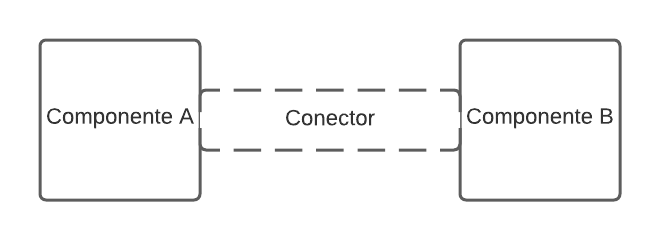
\includegraphics[scale=0.78]{cap_arquitectura/images/conector}
  \caption{Ejemplo de comunicación de dos componentes a través de un conector.}
  \label{fig:componentesYConectorEjemplo}
\end{figure}

Internamente, los conectores están compuestos por uno o más \textbf{conductos} o canales. A través de estos se lleva a cabo la comunicación entre los componentes. Hay una gran variedad de conductos posibles: comunicación interproceso, a través de la red, etc. Clasificamos los conectores según la complejidad de los canales que utilizan \cite{mehtaTaxonomySoftwareConnectors2000}:

\pagebreak

\begin{itemize}
    \item \textbf{Conectores simples}: solo cuentan con un conducto, sin lógica asociada. Son conectores sencillos. Suelen estar ya implementados en los lenguajes de programación. Por ejemplo: una llamada a función en un programa o el sistema de entrada / salida de ficheros.

    \item \textbf{Conectores complejos}: cuentan con uno o más conductos. Se definen por composición a partir de múltiples conectores simples. Además, pueden contar con funcionalidad para manejar el flujo de datos y/o control. Suelen utilizarse importando \emph{frameworks} o librerias. Por ejemplo: un balanceador de carga que redirige peticiones a los nodos.
\end{itemize}

Por tanto, cuando hayamos decidido que dos componentes necesitan comunicarse, es momento de evaluar qué mecanismo de comunicación es más adecuado. Basándonos en nuestros requisitos, la arquitectura ya definida, y los mecanismos de despliegue que queremos usar, elegimos el conector apropiado. Podemos orientarnos con taxonomías como la de \cite{mehtaTaxonomySoftwareConnectors2000}.

\subsubsection{Forma}

\textcolor{red}{TODO:  - ¿Borrar?  Innecesario}

\subsubsection{Justificación}

\textcolor{red}{TODO:  - ¿Borrar?  Innecesario}

Una vez definidos los componentes, los conectores y las relaciones entre ellos, tendremos una representación del sistema. Pero se trata de una imagen incompleta. No cuenta con ciertos detalles del contexto que nos ayudan a entenderlo mejor. Un ejemplo podría ser qué alternativas se consideraron y por qué se descartaron en favor de la elegida. Tampoco contamos con detalles minuciosos que puedan guiar mejor la implementación.

Es decir, requerimos de un concepto adicional para describirlos en nuestra arquitectura: se trata de la \textbf{justificación}. \cite{perryFoundationsStudySoftware1992} Nos aporta detalles más precisos sobre el sistema que no se pueden representar como elementos o forma.

\subsection{Estilos arquitectónicos}

\textcolor{red}{TODO:  - ¿Borrar?  Innecesario}

\textcolor{red}{Podemos agrupar decisiones principales.}

\section{Arquitectura de la solución}

Como comentamos en el capítulo \ref{chap:introduccion}, el objetivo del trabajo es transformar un servicio monolítico en un sistema distribuido basado en microservicios. Se trata de un cambio arquitectónico importante. Queremos por tanto diseñar una estrategia ingenieril para llevar a a cabo la migración; teniendo en cuenta las particularidades del sistema.

El servicio en cuestión implementa un \textbf{bucle de control MAPE-K}\cite{ibmcorporationArchitecturalBlueprintAutonomic2006,fonsServiciosAdaptivereadyPara2021}, que ya describimos en la sección \ref{sub:bucles-mapek}.

En esta sección presentaremos nuestra propuesta arquitectónica para adaptar el bucle para entornos en la nube.

\textcolor{red}{Buscar libros de descomposición de monolitos en microservicios.}

\subsection{Distribución de los componentes}

Actualmente, el bucle está muy acoplado a los modelos de sus recursos manejados. Todo corre bajo el mismo proceso: el bucle, los monitores, sus reglas de adaptación y demás elementos específicos de la solución\dots Ese proceso solo podrá manejar aquellos sistemas cuyos módulos tenga cargados. En la figura \ref{fig:bucle-mapek2} presentamos otra vista de la arquitectura del bucle.

\begin{figure}[htb]
  \centering
  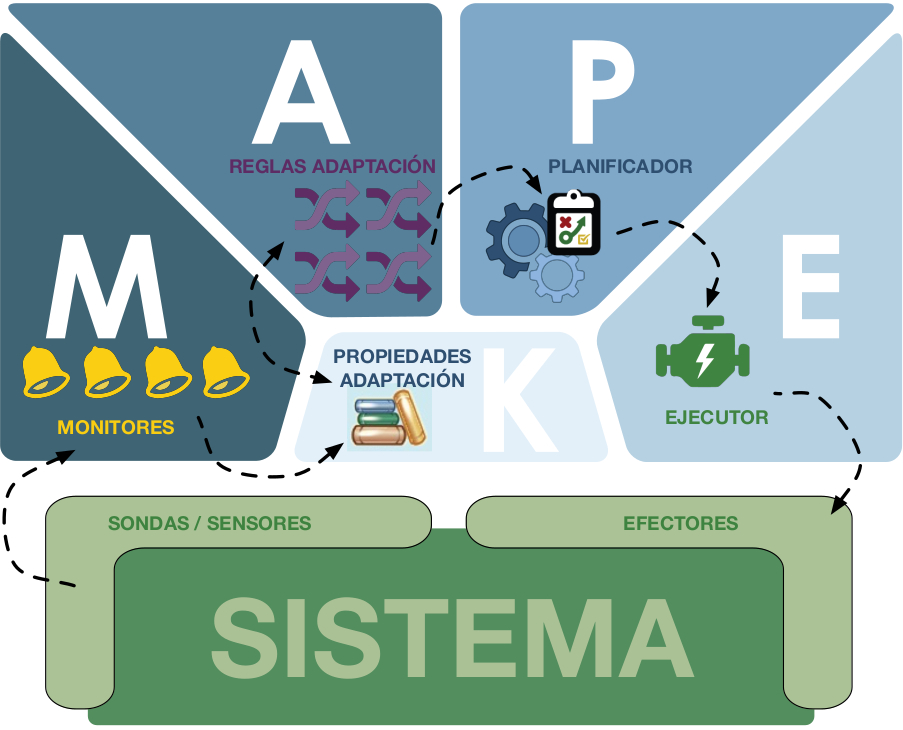
\includegraphics[scale=1.15]{cap_introduccion/images/bucle-mape-k}
  \caption[Arquitectura de un Bucle MAPE-K. Podemos apreciar el flujo de información y de control a lo largo de las etapas del bucle.]{Arquitectura de un Bucle MAPE-K. Podemos apreciar el flujo de información y de control a lo largo de las etapas del bucle. Obtenida de \cite{fonsEspecificacionSistemasAutoadaptativos2021}}
  \label{fig:bucle-mapek2}
\end{figure}

Partimos entonces el objetivo de desacoplarlo. Así, podremos desplegarlo y usarlo de forma agnóstica al recurso manejado. La misma infraestructura podrá aprovecharse para manejar varios sistemas simultáneamente (\emph{multi-tennancy}). La idea es implementarlo a nivel de sistema\cite{mendoncaGeneralityVsReusability2018}, por lo que se desplegará al mismo con los microservicios del recurso manejado.

Como veremos a continuación, cada uno de sus componentes es candidato a convertirse en un microservicio individual.

Por la descripción de ambos componentes, vemos que existe una clara división de dominios y responsabilidades. Esto nos ayuda a determinar que ambos componentes pueden desplegarse por separado. \textcolor{red}{REFERENCIA 'Building Microservices' Sam Newman}

Por suerte, partimos de un sistema existente, con una arquitectura bien definida y documentada. Conocíamos el rol de cada uno de los componentes del servicio y sus requisitos. Asi que, el primer problema al que nos enfrentamos estaba relacionado con la distribución de los servicios. ¿Cómo definimos las fronteras entre cada uno de ellos? ¿Qué componentes debe abarcar cada microservicio?

La primera decisión que tomamos fue desacoplar el bucle de los sistemas. Buscábamos desarrollar microservicios agnósticos a la solución manejada. Por ello, vamos a identificar distintos \textbf{niveles de componentes} \textcolor{red}{Imagen que separa el bucle de la lógica de la solución.} Esto nos permitiría dar servicio a varios sistemas distintos con la misma infraestructura. Multi-tennancy.

Otra decisión que tomamos fue separar cada etapa del bucle en su propio servicio. Así podríamos independizarlas y escalarlas individualmente.

Una vez determinadas las fronteras entre los microservicios, hemos definido los componentes de nuestro sistema.

\begin{figure}[htb]
  \centering
  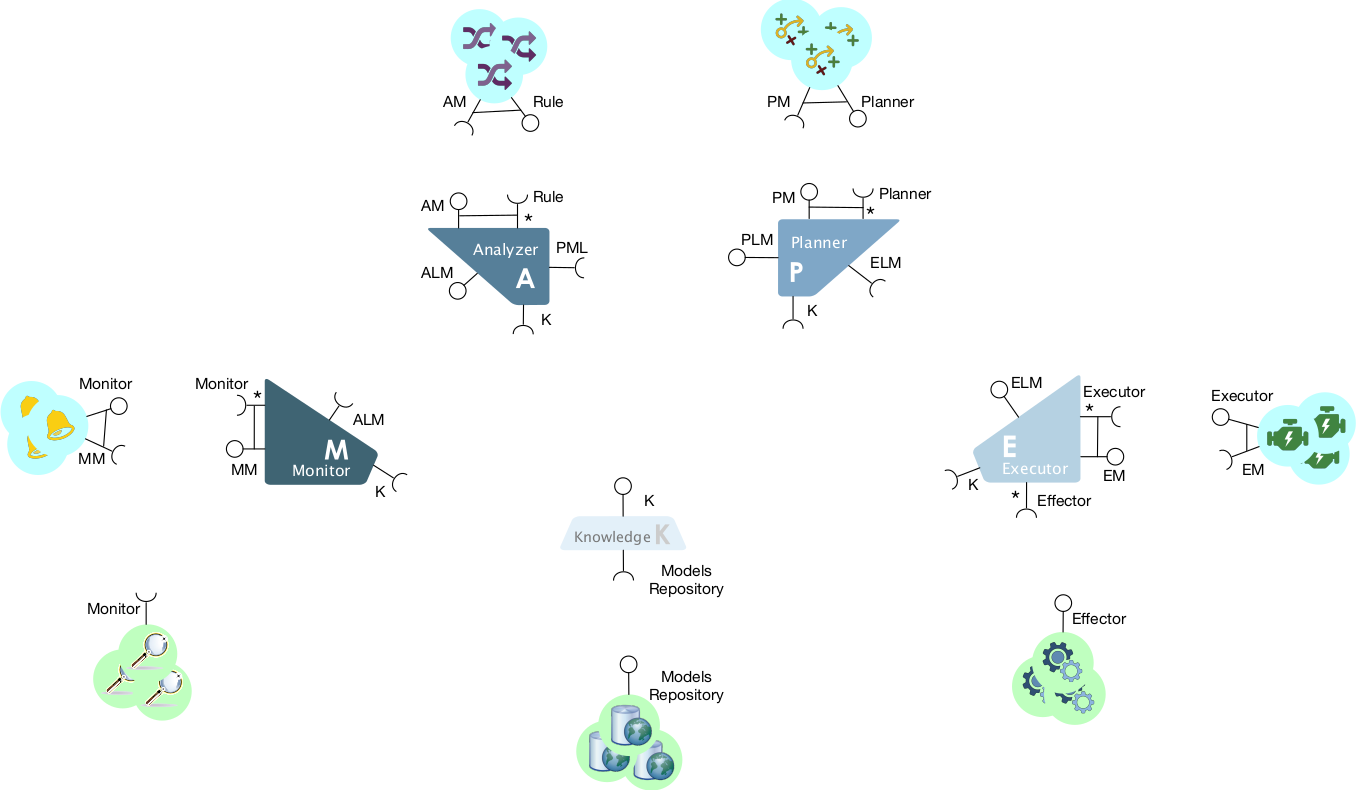
\includegraphics[scale=0.3]{cap_arquitectura/images/mape-k-microservices}
  \caption{Diagrama con los componentes que forman nuestra arquitectura distribuida}
  \label{fig:mape-k-microservices}
\end{figure}

\textcolor{red}{Figura \ref{fig:mape-k-microservices}: Agrupar los servicios para poder aumentar zoom y hacerlo más legible. Añadir línea de divisón entre la capa del bucle y el dominio del recurso manejado.}

\subsection{Conectando los servicios}

El siguiente problema al que nos enfrentamos está relacionado con la comunicación: si dividimos estos componentes en microservicios, ¿cómo hacemos para que se comuniquen? Hay que tener en cuenta que estos pueden estar desplegados y replicados en distintas máquinas. No podemos asumir que están en el mismo \emph{host}.

Aprovechando la separación entre bucle de control y el dominio del recurso, investigamos posibles arquitecturas. Nos decantamos por \textbf{arquitecturas de servicios jerarquizados}. Queríamos explotar esta separación para mantener al bucle aislado del dominio de la solución. Dimos con el estilo arquitectónico C2 (\emph {components and connectors})\cite{taylorComponentMessagebasedArchitectural1996a, UCISoftwareArchitecture}, en el que nos hemos inspirado.

\subsubsection{Jerarquías de microservicios: Arquitectura C2 y arquitectura limpia}

Este estilo organiza sus componentes en jerarquías o capas: cada servicio se encuentra en un nivel determinado, según su nivel de abstracción. En las capas inferiores, se encuentran los servicios más externos, más ''acoplados'' al entorno. Por ejemplo, aquellos servicios que requieran de acceder al sistema de ficheros, estarían en esta capa. Por otro lado, en las capas superiores se encuentran los servicios en niveles de abstracción superior, que dependen lo mínimo del entorno.

En cuanto a la comunicación, un componente solo debe contactar con sus vecinos inmediatos (en una capa superior o inferior). Esto evita que el servicio pueda contactar con otras capas, limitando su alcance y su conocimiento del despliegue del sistema. Además, dentro del mismo nivel no pueden contactar entre ellos. Según la dirección de la comunicación, se emplean mecanismos distintos (figura \ref{fig:C2-arch-example}):

\begin{itemize}
  \item \textbf{Peticiones} (\emph{requests}): Se trata de solicitudes a un servicio para que ejecute una acción. Un componente se comunica directamente con un vecino en una capa superior. La petición viaja de ''fuera hacia dentro'' en cuanto al nivel de abstracción. Por ejemplo, una petición de un cliente a un servicio web podría estar bajo esta categoría.

  \item \textbf{Notificaciones}: Representan eventos ocurridos en el sistema. Un componente de más arriba en la jerarquía (más interno) envía un mensaje hacia abajo, sin especificar receptor. Todos los servicios por debajo lo recibirán, y decidirán si tratarlo o no. Esto evita que nuestro servicio se acople a aquellos que están por debajo (son más concretos). Un ejemplo sería notificar al resto de servicios sobre la creación de un nuevo usuario.
\end{itemize}

\begin{figure}[htb]
  \centering
  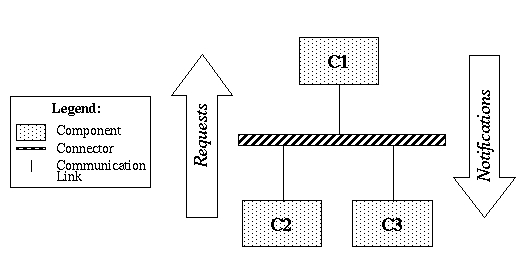
\includegraphics[scale=0.45]{cap_arquitectura/images/c2SampleArch}
  \caption[Ejemplo del estilo arquitectónico C2 (\emph{Components and Connectors})]{Ejemplo del estilo arquitectónico C2 (\emph{Components and Connectors}). \cite{UCISoftwareArchitecture}}
  \label{fig:C2-arch-example}
\end{figure}

Basándonos en este estilo, definimos las capas de nuestro sistema. Esto nos permitió dividir los microservicios en niveles y elegir los conectores más adecuados para cada tipo de comunicación.

Distinguimos cuatro niveles distintos, de menor nivel de abstracción a mayor:

\begin{itemize}
  \item \textbf{Nivel del recurso manejado}: En este nivel se encuentran las sondas y efectores. Son los elementos que tienen más contacto con el recurso manejado. Hacen de intermediarios entre este y el resto del bucle, para reducir su acoplamiento.

  \item \textbf{\textcolor{red}{Nivel de específico solución}}: En esta capa se encuentran componentes del bucle específicos para el dominio del recurso manejado. Monitores específicos, reglas de adaptación... No los incluimos en el mismo nivel que las sondas y efectores porque necesitamos comunicar con ellos. Además que guardan más relación con el bucle que con el recurso manejado.

  \item \textbf{Nivel del bucle}: Aquí se encuentran los servicios de las etapas del bucle: servicio de monitorización, análisis, planificación y ejecución. Esta capa debe ser agnóstica al dominio de los recursos manejados. Además, actúa como intermediario entre los servicios de la solución y el conocimiento. Limitan cómo acceder a él.

  \item \textbf{Conocimiento}: Es la capa más interna y la base de la arquitectura. No depende de ningún otro componente, por lo que tiene el nivel de abstracción más alto. Todos los componentes del nivel del bucle dependen de ella para funcionar.

\end{itemize}

Habiendo definido esta jerarquía, vimos ciertas similitudes con arquitecturas \emph{domain driven}, como \emph{Clean Architecture}. \cite{martinChapter22Clean2018} En ella, el sistema se organiza en base a una \textbf{regla de dependencia}: \emph{''la dependencia entre los componentes solo puede apuntar hacia dentro, hacia políticas de alto nivel''}. Es decir, la arquitectura se organiza en capas concéntricas. En el centro se encuentra el dominio, con el mayor nivel de abstracción. Este no tiene dependencias con ninguna capa exterior. Por otro lado, cada capa más externa tiene dependencias sólo con la capa a la que envuelve. Sólo puede comunicarse con componentes dentro de esta.

Basándonos en la descripción anterior, nuestra capa central será la del conocimiento. A partir de ahí, cada nivel superior dependería de aquel al que ''envuelve'': el bucle al conocimiento, la solución al bucle...Por tanto, para que nuestra arquitectura sea más comprensible, optamos por representarla los diagramas de \emph{Clean Architecture} para representarlo. En la figura \ref{fig:clean-mapek-architecture} mostramos el resultado:

\begin{figure}[htb]
  \centering
  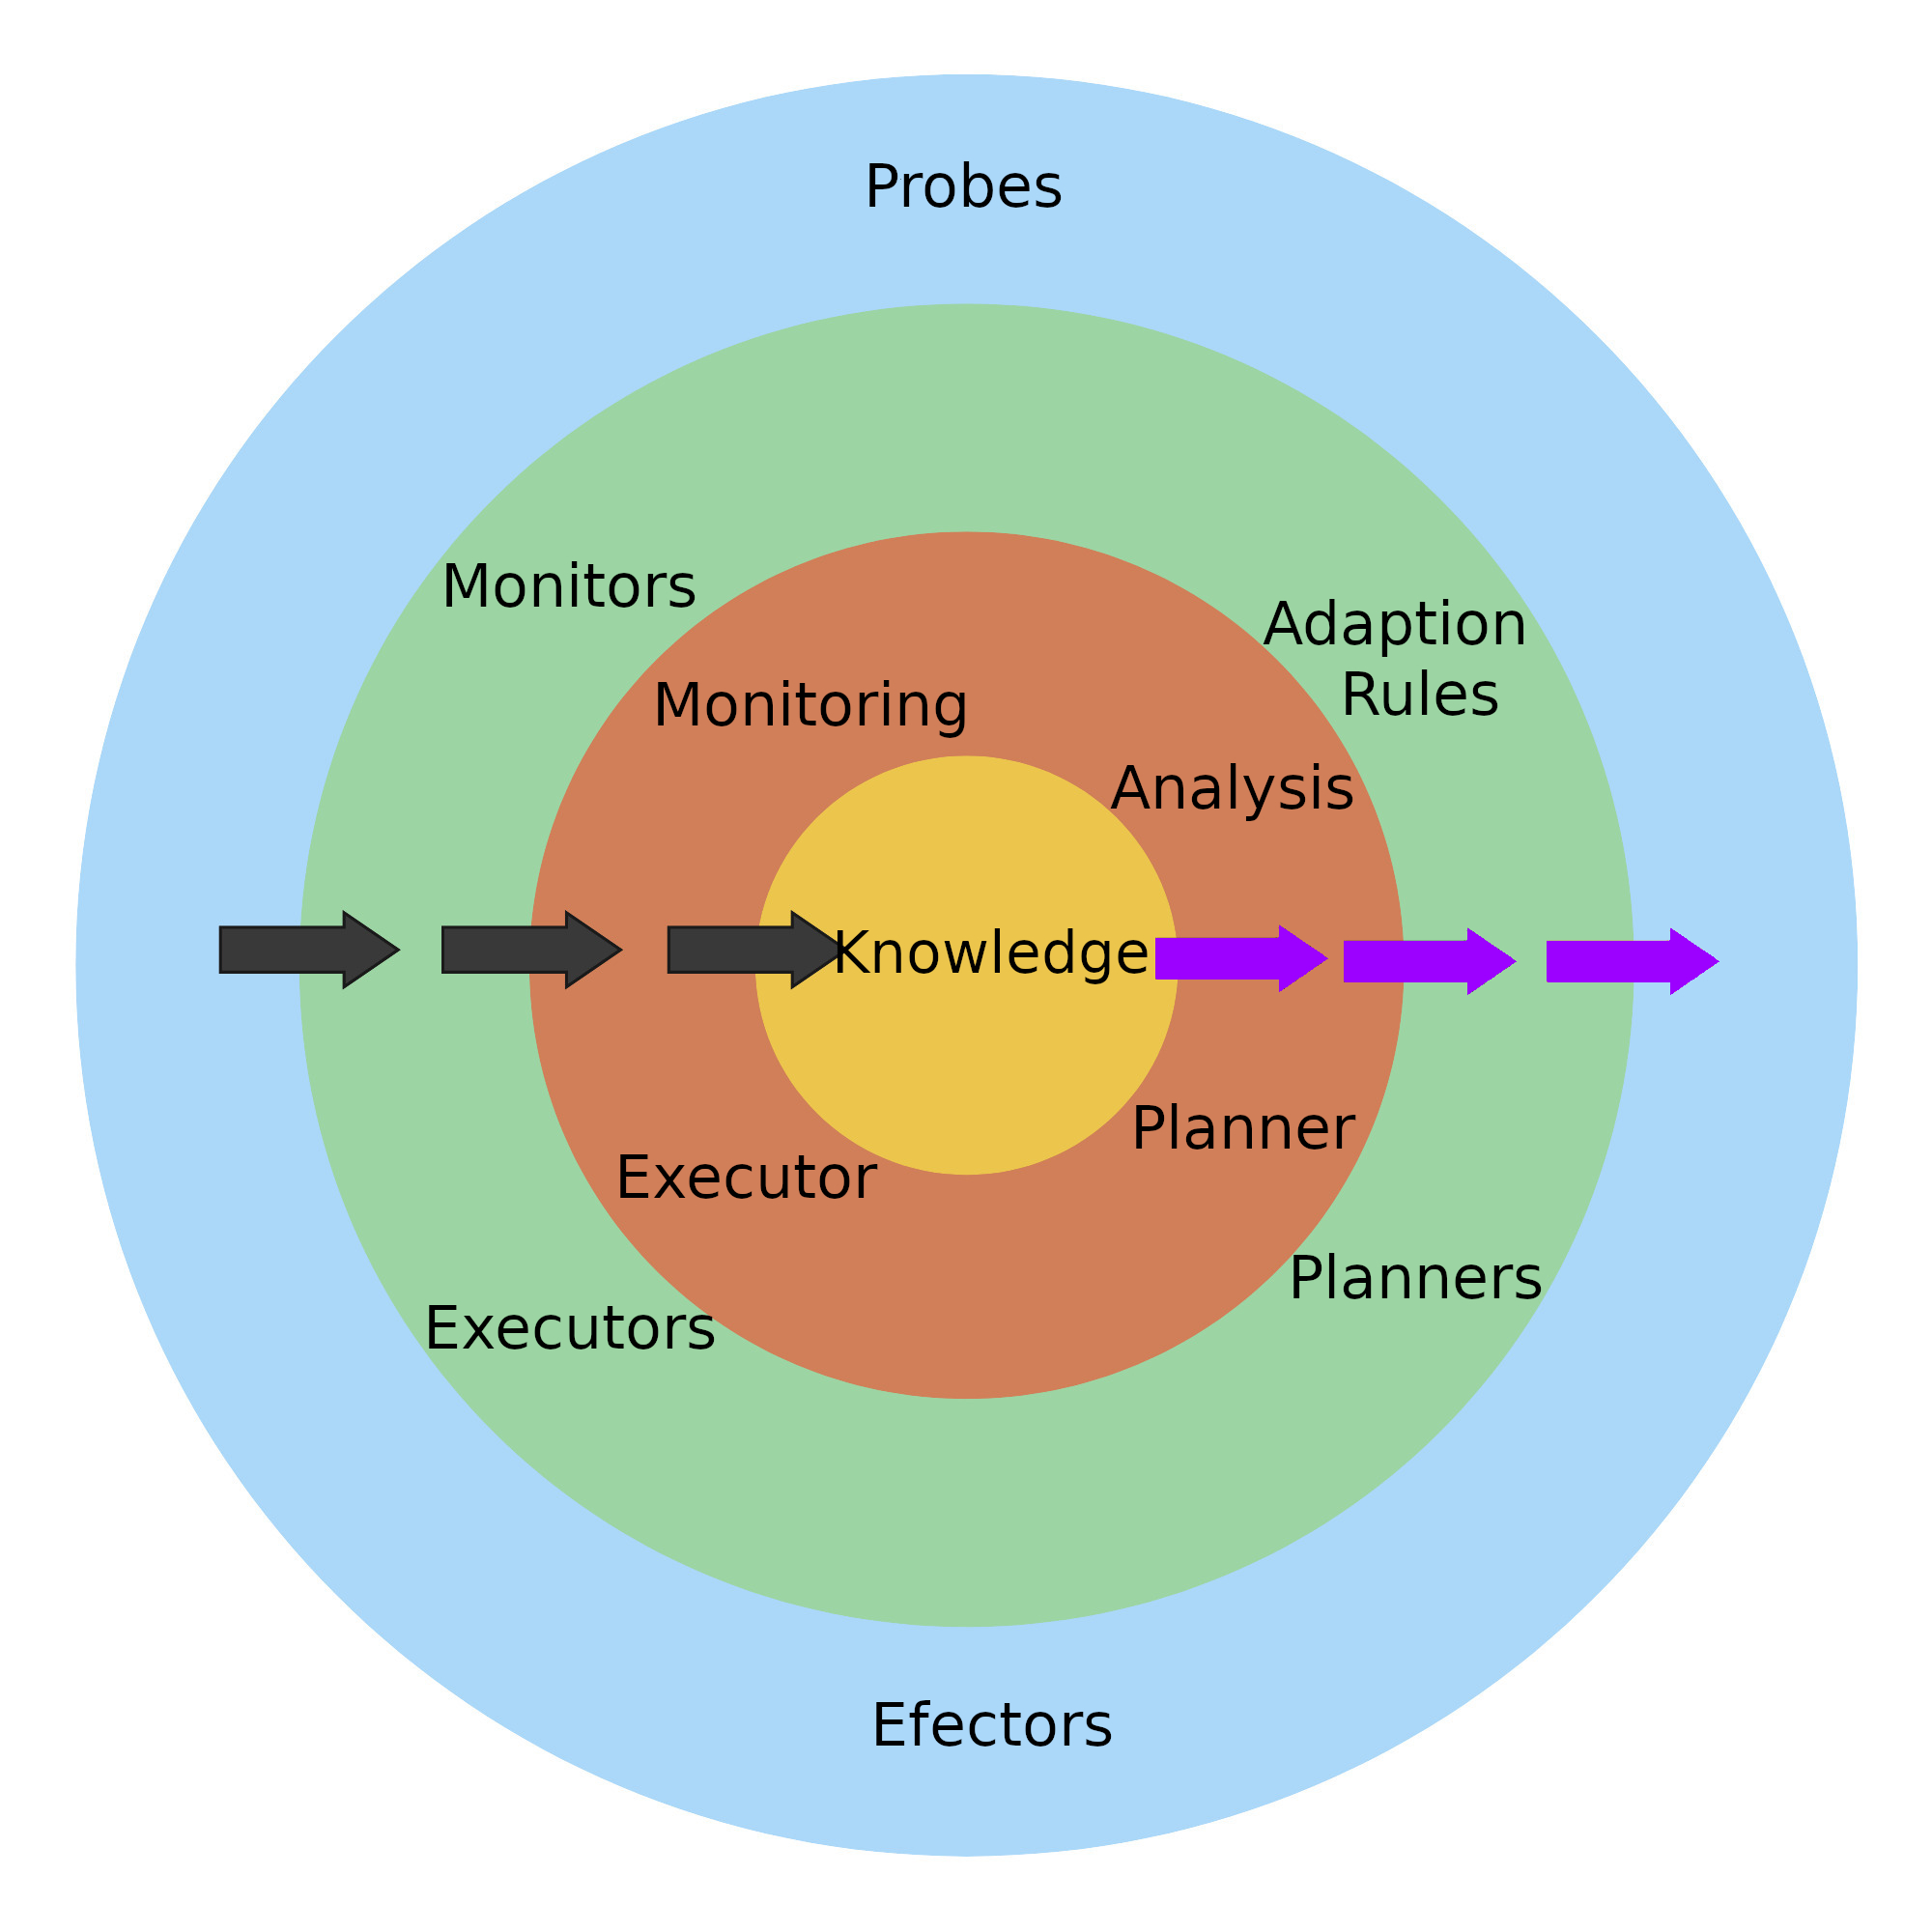
\includegraphics[scale=0.45]{cap_arquitectura/images/clean-arch-2-MAPEK-style-small}
  \caption[Representación de nuestra propuesta arquitectónica. Inspirado en Arquitectura Limpia (\emph{Clean Architecture}). Las flechas negras representan las peticiones, y las moradas, las notificaciones.]{Representación de nuestra propuesta arquitectónica. Inspirado en Arquitectura Limpia (\emph{Clean Architecture}). Las flechas negras representan las peticiones, y las moradas, las notificaciones. \footnotemark }
  \label{fig:clean-mapek-architecture}
\end{figure}

\footnotetext{Imagen original de arquitectura limpia obtenida de: \url{https://threedots.tech/post/ddd-cqrs-clean-architecture-combined/}}

\subsubsection{Definiendo los mecanismos de comunicación}

Como comentamos antes, vamos a inspirarnos en los mecanismos de comunicación descritos por C2: las peticiones y notificaciones. Pero, durante nuestra etapa de prototipado, nos dimos cuenta que estos no cubren todas nuestras necesidades. Hay dos casos que no están contemplados: la comunicación del módulo de análisis con el planificador, y la del planificador con el ejecutor. Ambos módulos se encuentran en la misma capa. Y, como dependen del conocimiento, no podemos moverlos a una superior para utilizar notificaciones.

\textcolor{red}{Las notificaciones no nos sirven, ya que la comunicación es entre dos módulos específicos. Aunque nos interesa el desacoplamiento entre módulos que ofrecen. Las peticiones tampoco casan del todo, ya que requerimos desacoplar los módulos. Deberían mantener su independencia en el mayor grado posible.} Por ello, requerimos de un tercer patrón de comunicación. Una combinación de ambos: las peticiones asíncronas.

Los tres patrones de comunicaciones que usaremos entonces son:

\begin{itemize}
  \item \textbf{Peticiones síncronas}: Comunicaciones síncronas dirigidas a un servicio determinado. Solo permitidas entre servicios de una capa más externa a un servicio en la capa interior adyacente.

  \item \textbf{Peticiones asíncronas}: Comunicaciones asíncronas dirigidas a un tipo de servicio determinado. Se trata de peticiones de trabajo asíncronas: se envían y el destinatario lo procesará cuando pueda. El cliente continuará su ejecución, sin esperar respuesta. \emph{fire and forget}.

  Para evitar el acoplamiento entre los componentes, deberemos buscar un conector que permita enviar el mensaje sin conocer específicamente al destinatario.

  Este mecanismo de comunicación solo está permitido entre elementos del mismo nivel.

  \item \textbf{Notificaciones}: Comunicaciones asíncronas no dirigidas. El servicio publica un evento que potencialmente recibirán todos los servicios en la capa exterior adyacente. El cliente lo envía y continua su ejecución, sin esperar respuesta.
\end{itemize}

\subsubsection{Conectores}

Una vez determinadas las necesidades de comunicación de nuestro sistema, debemos buscar los conectores adecuados. Seguimos la estrategia descrita en \cite{taylorSoftwareArchitectureFoundations2009} para elegir conectores; y nos basamos en los patrones de comunicación en sistemas distribuidos descritos en \cite{newmanBuildingMicroservicesDesigning2021}.

Comenzamos investigando las peticiones síncronas. Tomemos por ejemplo la comunicación entre el servicio de monitorización (\emph{monitoring service}) y el servicio de conocimiento (\emph{knowledge service}). Recordemos que el servicio de conocimiento almacena todas las propiedades de adaptación. El resto de servicios necesitan consultarlas y actualizarlas durante su funcionamiento. En la figura \ref{fig:monitor-knowledge-initial} representamos inicialmente ambos componentes y un conector, sin especificar de qué tipo será.

% TODO: Cambiar por imagen de componentes, que ofrezcan y requieran interfaces.
\begin{figure}[htb]
  \centering
  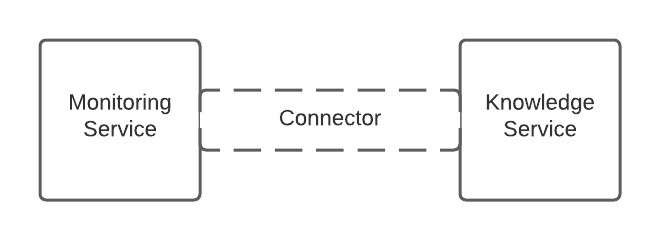
\includegraphics{cap_arquitectura/images/Monitor-Knowledge-Initial-Connector}
  \caption{Boceto inicial: queremos conectar el servicio de monitorización con la base de conocimiento para poder leer propiedades de adaptación.}
  \label{fig:monitor-knowledge-initial}
\end{figure}

El siguiente paso es identificar qué interacciones debe existir entre ambos componentes. En este caso, el servicio de monitorización debe contactar con el servicio de conocimiento para leer y actualizar el valor de las propiedades.Por tanto, existen operaciones de lectura y escritura de los datos. Además, como es una comunicación ''descendente'' (\emph{monitoring service} está en la capa superior), el patrón a utilizar serán las peticiones síncronas.

Ahora, debemos identificar qué \textbf{tipos de conector} serían adecuados para este patrón. Sabiendo que hemos optado por una arquitectura distribuida, la elección se simplifica: los servicios pueden estar desplegados en máquinas distintas, por tanto el paso de mensajes será a través de la red.

Conociendo esto, en lugar de recurrir a la taxonomía que lista \cite{mehtaTaxonomySoftwareConnectors2000}, optamos por consultar las estrategias de comunicación habituales para sistemas distribuidos descritas en \cite{newmanBuildingMicroservicesDesigning2021}. Se trata de cuatro mecanismos distintos: Invocación a métodos remotos (\emph{Remote Procedure Call}), APIs REST, consultas con GraphQL o \emph{brokers} de mensajería. Tuvimos que evaluarlos mediante un análisis de \emph{trade-offs} para determinar las ventajas y desventajas de cada uno.

\textcolor{red}{Smart endpoints, dumb pipes: https://simplicable.com/new/smart-endpoints-and-dumb-pipes}

\textbf{Invocación de métodos remotos} o (\emph{\textbf{Remote Procedure Call}}): Esta patrón se basa en el estilo cliente-servidor. Un servidor expone una serie de funciones que el cliente puede invocar mediante peticiones a través de la red. Estas peticiones incluyen el nombre de la función a ejecutar y sus parámetros. Al finalizar la ejecución, el servidor puede devolver su resultado, si lo hubiera. Existen varios protocolos que implementan este mecanismo como gRPC o SOAP.

Una evolución de RPC suele emplearse en la programación orientada a objetos: el paradigma de \textbf{objetos distribuidos}. \cite{tanenbaumChapter10Distributed2007} En este caso, el programa cliente puede interactuar con objetos en servidores remotos como si fueran locales. Esta interacción se realiza a través de objetos que actúan como \emph{proxies}, abstrayendo de la llamada al servidor.

Los \emph{proxies} ofrecen una interfaz para que el cliente invoque sus métodos localmente. Internamente, estos métodos realizan una llamada al servicio remoto donde se encuentra el objeto realmente. El servidor remoto procesa la petición y nos devolverá un resultado. Así, abstraen al cliente de todo este proceso de comunicación. En la figura \ref{fig:rpc-distributedobjects} tenemos un esquema de este mecanismo.

\begin{figure}[htb]
  \centering
  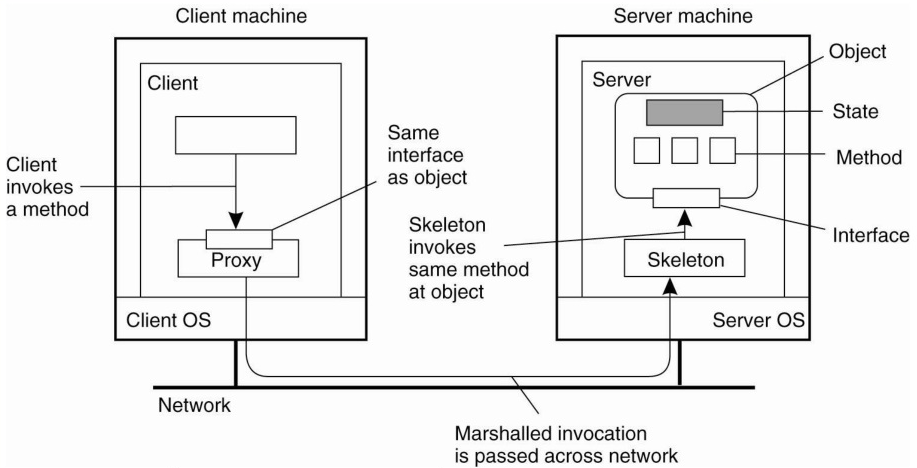
\includegraphics[scale=1.5]{cap_arquitectura/images/rpc-distributedobjects}
  \caption[Funcionamiento del sistema de objetos distribuidos]{Funcionamiento del sistema de objetos distribuidos. \cite{tanenbaumChapter10Distributed2007}}
  \label{fig:rpc-distributedobjects}
\end{figure}

\begin{itemize}
  \item \textbf{Ventajas}:
  \begin{itemize}
    \item Permite distribuir la carga de procesamiento del sistema. Esto puede ayudar para escalar la aplicación.

    \item Abstrae al cliente de la interacción con un servidor remoto. Le resulta prácticamente indistinguible de un objeto local.

    \item \textcolor{red}{Los \emph{proxies} o (\emph{stubs} en la terminología de RPC) suelen generarse a partir de un contrato que define qué operaciones ofrecen estos objetos. Por ejemplo: SOAP con WDSL, gRPC; o en el caso de objetos distribuidos, Java RMI.} ¿Y la ventaja?
  \end{itemize}

  \item \textbf{Desventajas}:
  \begin{itemize}
    \item No se puede abstraer completamente al cliente de las llamadas a través de la red. Pueden darse errores que no ocurrirían durante una invocación de un método sobre un objeto local. Por ejemplo, que el servidor no esté disponible. \cite{jausovecFallaciesDistributedSystems2020}

    \item Dificulta la integración con otras aplicaciones. Cada servicio ofrece sus propias funciones distintas. No están estandarizadas.

    \item Si adoptamos sistemas como Java RMI, nuestro sistema se acopla a esa tecnología concreta. \cite{newmanBuildingMicroservicesDesigning2021}. Nos quita flexibilidad en cuanto a qué otras tecnologías podemos utilizar en nuestra arquitectura.

    \item El cliente debe actualizarse y recompilarse con cada cambio en el esquema del servidor. Esto puede ser problemático para casos donde tenemos que desplegar una actualización para que nuestros clientes puedan continuar utilizando la aplicación.
  \end{itemize}
\end{itemize}

\textbf{\emph{Representational State Transfer} (REST)}: Se basa también en el estilo arquitectónico cliente-servidor, pero con ciertas restricciones adicionales. \cite{taylorSoftwareArchitectureFoundations2009} Su concepto principal son los \textbf{recursos}: cualquier elemento sobre el que la API pueda ofrecernos información; y que pueda tener asociado un identificador único (una URI). \cite{richardsonRESTfulWebServices2007} Por ejemplo, podrían ser las entidades del dominio que gestiona nuestro servicio: usuarios, mediciones de temperaturas\dots

Las acciones que podemos ejecutar sobre los recursos (leer, crear, actualizar, \dots) las define el protocolo de comunicación sobre el que se implemente. Gracias a esto, la API que pueden ofrecer los servicios REST es común. Solo cambia el ``esquema de los datos``, los tipos de recursos que ofrecen. Esto facilita enormemente la integración con otros servicios. \cite{nallyRESTVsRPC2018} La implementación más habitual es sobre el protocolo HTTP. Define métodos estandarizados como \emph{GET} para las lecturas, \emph{PUT} para las actualizaciones, etc.

\begin{itemize}
  \item \textbf{Ventajas}:

  \begin{itemize}
    \item \textbf{\emph{Stateless}}: El servidor no mantiene el estado de la sesión del cliente. Esto permite que cada petición sea independiente de las demás.

    \item \textbf{Escalable}: Como las sesiones deben ser \emph{stateless}, podremos replicar nuestro servicio y que distintas instancias puedan atender las peticiones que surjan durante una misma sesión.

    \item \textbf{API Sencilla}: Solo hay que implementar unos pocos métodos estándar para interactuar con la API.

    \item \textbf{Comunicación síncrona}: Es el mecanismo ideal para comunicaciones síncronas, donde el cliente requiere la respuesta del servicio para poder continuar con su procesamiento. También podemos dar soporte a para comunicaciones \emph{fire and forget}, donde el cliente envía un mensaje y no espera ninguna respuesta a su petición.

    \item \textbf{Interoperabilidad}: Ampliamente utilizado en servicios de Internet. Es ideal para que clientes externos contacten con nuestro sistema mediante peticiones síncronas. \cite{newmanBuildingMicroservicesDesigning2021}

    \item \textbf{Generación de clientes}: Para facilitar la comunicación con APIs REST, podemos generar librerias cliente utilizando el estándar OpenAPI. Lo explicaremos con maś detalle en la sección \ref{chap:OpenAPI}.
  \end{itemize}

  \item \textbf{Desventajas}:

  \begin{itemize}
    \item \textbf{Dirigida}: Necesitamos conocer de antemano la ubicación del servidor al que queremos hacer una petición.

    \item \textbf{Rendimiento}: El rendimiento es peor comparado con mecanismos RPC. El tamaño de un mensaje HTTP serializado en XML o JSON es mayor que si estuviera en un formato binario.

    \item \textbf{API Sencilla}: También es una desventaja. Hay operaciones complejas que pueden ser difíciles de representar con los métodos ofrecidos por el protocolo de comunicación. Pueden requerir más tiempo de diseño, o incluso, ser implementados siguiendo el patrón RPC.
  \end{itemize}
\end{itemize}

\textbf{GraphQL}\footnote{Página oficial: \url{https://graphql.org/}} \textcolor{red}{AMPLIAR}: Se trata de un protocolo de consultas. Permite a los clientes ejecutar consultas personalizadas sobre los datos de un servidor. No necesitan de lógica específica para ejecutarla. De esta forma, el cliente puede obtener toda la información que necesita. Reduce el número de peticiones ejecutadas. También evita traerse datos innecesarios.

\begin{itemize}
  \item \textbf{Ventajas}:

  \begin{itemize}
    \item \textbf{Ideal para móviles}: Gracias a que reduce la cantidad de llamadas, es ideal para entornos donde queremos optimizar el uso de red.

    \item \textbf{Rendimiento}: Ofrece un mayor rendimiento comparado con otras alternativas que no ofrezcan un endpoint ya implementado. Y debamos obtener la misma información por composición, haciendo varias llamadas.
  \end{itemize}

  \item \textbf{Desventajas}:

  \begin{itemize}
    \item \textbf{Solo permite lecturas}: Es un lenguaje de consultas. No tiene comandos que permita escrituras.

    \item \textbf{Solo permite lecturas síncronas}:

    \item \textbf{Exponemos datos a la red}:

    \item \textbf{Problemas de rendimiento}: El cliente puede hacer consultas muy pesadas que penalicen el rendimiento de la base de datos sobre la que opera nuestro servicio.
  \end{itemize}
\end{itemize}

\textbf{\foreign{english}{Brokers} de mensajería}: Es un mecanismo de \textbf{comunicación asíncrona} muy popular. Sobre todo en arquitecturas basadas en eventos. Contamos con un servicio que actúa como intermediario, el \emph{broker}. Este gestiona la comunicación entre los servicios del sistema. \cite{newmanBuildingMicroservicesDesigning2021} Hay varias estrategias de comunicación posibles: colas de trabajo, \emph{publish-suscribe}, híbrida\dots

Tomemos por ejemplo las \textbf{colas de trabajo}. \cite{royChapterMessagePatterns2017} Es una estrategia para implementar comunicaciones asíncronas dirigidas. Nos permiten desacoplar la comunicación entre componentes usando colas de mensajería como intermediarias. Para ello, un servicio, el productor, publica mensajes en la cola. Estos mensajes representan peticiones de trabajo que pueden ser costosas de procesar. Un servicio, el trabajador, estará la escucha de los mensajes que llegan y los irá consumiendo. Estos mensajes se procesan siguiendo un orden FIFO (\emph{first in, first out}). En la figura \ref{fig:work-queues} mostramos un ejemplo con dos consumidores, a la escucha de la misma cola.

\begin{figure}[htb]
  \centering
  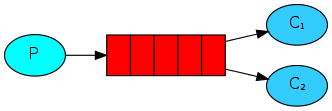
\includegraphics[scale=0.65]{cap_arquitectura/images/work-queues}
  \caption[Representación de las colas de trabajo. Ejemplo de comunicación asíncrona dirigida.]{Representación de las colas de trabajo. Ejemplo de comunicación comunicación asíncrona dirigida. \footnotemark }
  \label{fig:work-queues}
\end{figure}

\footnotetext{Imagen obtenida de: \url{https://www.rabbitmq.com/tutorials/tutorial-two-dotnet.html}}

Otra estrategia posible es \foreign{english}{publish-suscribe}: sirve para implementar comunicación \emph{multicast}. Se basa en el uso de \textbf{temas} o \textbf{\foreign{english}{topics}}: categorías de mensajes que pueden resultar de interés. Un servicio (el productor) envía un mensaje al \foreign{english}{broker}, indicando que pertenece a un tema determinado. El \emph{broker} recibe el mensaje y se encarga de reenviarlo a todos los servicios subscritos a este tema en concreto. \cite{rabbitmqPublishSubscribeDocumentation} En la figura \ref{fig:publish-subscribe} tenemos un ejemplo de esta estrategia.

\textcolor{red}{Describir fanout}
\textcolor{red}{Describir exchanges}

\begin{figure}[htb]
  \centering
  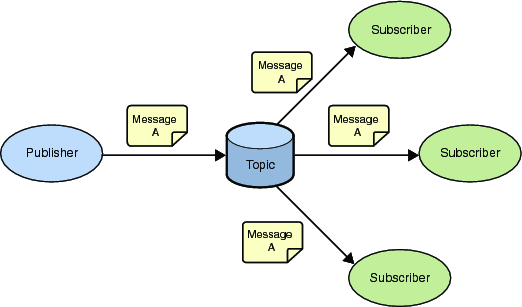
\includegraphics[scale=0.5]{cap_arquitectura/images/publish_subscribe}
  \caption[Estrategia \emph{publish/suscribe}: el \emph{broker} actúa como intermediario en la comunicación \emph{multicast}.]{Estrategia \emph{publish/suscribe}: el \emph{broker} actúa como intermediario en la comunicación \emph{multicast}. Imagen obtenida de \footnotemark}
  \label{fig:publish-subscribe}
\end{figure}

\footnotetext{Java Messaging Service: \url{https://docs.oracle.com/cd/E19509-01/820-5892/ref_jms/index.html}}

La mayor ventaja de este estilo de comunicación es el \textbf{desacoplamiento} entre los servicios. \cite{korabUnderstandingMessageBrokers2017}
Ninguno de ellos necesita conocer detalles sobre cómo están desplegado los otros: su dirección, el número de instancias, si están activos en este momento, etc. Solo necesitan conocer el formato de los mensajes y la dirección del \emph{broker} para enviarlos o recibirlos.

\begin{itemize}
  \item \textbf{Ventajas}:

  \begin{itemize}
    \item \textbf{Comunicación asíncrona}: El servicio no necesita quedarse a la espera de una respuesta del servidor. Puede procesar otras operaciones hasta que se le notifique del resultado, si lo hubiera.

    \item \textbf{Desacoplamiento de los servicios}: Ni los productores ni los consumidores necesitan conocer el origen o destino de sus mensajes. Solo su formato y la dirección del \emph{broker}.

    \item \textbf{Envío garantizado de mensajes}: El \emph{broker} garantiza que el mensaje será entregado \emph{al menos} una vez al consumidor. Reintentará el reenvío hasta que se confirme su recepción.

  \end{itemize}

  \item \textbf{Desventajas}:

  \begin{itemize}
    \item \textbf{Requisitos de infraestructura}: Utilizar un \emph{broker} de mensajería puede incrementar la dificultad de nuestros despliegues. El \emph{broker} puede convertirse en un punto de fallo. Para operar de forma fiable, estos sistemas requieren de replicación. \cite{newmanBuildingMicroservicesDesigning2021}

    \item \textbf{Envío garantizado de mensajes}: Para poder garantizar el envío de un mensaje, el \emph{broker} puede recurrir a reenviarlo. Debemos diseñar nuestros sistemas de forma que estos mensajes duplicados sean descartados si ya han sido procesados.
  \end{itemize}
\end{itemize}

En la tabla \ref{tab:comparativa-mecanismos-comunicacion} presentamos un resumen de esta comparativa:

\begin{longtable}{|p{4.4cm} | c | c | c | c|}
  \hline
  & \textbf{RPC} & \textbf{REST} & \textbf{GraphQL} & \textbf{Broker mensajería} \\
  \hline
  \textbf{Tipo de comunicación entre componentes} & Directa & Directa & Directa & Directa y \emph{Multicast} \\
  \hline
  \textbf{Acoplamiento entre componentes} & Alto & Medio & Alto & Bajo \\
  \hline
  \textbf{Interoperabilidad} & Baja & Alta & Alta & Alta\footnotemark \\
  \hline
  \textbf{Comandos de lectura} & Sí & Sí & Sí & Sí \\
  \hline
  \textbf{Comandos de escritura} & Si & Sí & No & Sí \\
  \hline
  \textbf{Comunicación síncrona} & Sí & Sí & Sí & No \\
  \hline
  \textbf{Comunicación asíncrona} & No & Sí & No & Si \\
  \hline
  \caption{Comparativa de los mecanismos de comunicación.}
  \label{tab:comparativa-mecanismos-comunicacion}
\end{longtable}

\footnotetext{Depende de si tenemos control sobre los componentes que queremos integrar.}


--------------------------------------------------------------

Ahora analizaremos qué protocolo elegimos para cada mecanismo de comunicación.

\subsubsection{Peticiones síncronas}

De estas cuatro opciones, podemos descartar inmediatamente la opción de GraphQL. Se trata de un conector más orientado a las consultas de datos. En nuestro caso, necesitamos ejecutar también escrituras de los valores de las propiedades. Aunque podría ser interesante para consultas más avanzadas, utilizar dos protocolos de comunicación en paralelo aumentaría la complejidad de la arquitectura.

También optamos por descartar el \emph{broker} de mensajería. Como requerimos de comunicación directa, nos convenía que esta fuera síncrona. Para obtener propiedades del conocimiento, resultaba más sencillo de implementar mediante comunicación síncrona.

Finalmente, hay que tener en cuenta que una de nuestras prioridades es la \textbf{interoperabilidad}: es una API expuesta ''hacia fuera'', hacia una capa más externa; prima por tanto la compatibilidad con cualquier tipo de cliente. Descartamos entonces RPC, dado que nos acoplaría a una tecnología concreta y a APIs no estándares.

Terminamos por tanto decantándonos por implementar la comunicación utilizando un conector REST sobre HTTP. Implementaremos ambas funciones mediante \emph{endpoints} HTTP. Su especificación se detalla a continuación en las tablas \ref{tab:especificacion-get-property} y \ref{tab:especificacion-put-property}.

\newsavebox\getpropertyrequestbox
\begin{lrbox}{\getpropertyrequestbox}
  \begin{minipage}[t]{1in}
    \begin{verbatim}
Request:
HTTP GET property/currentTemperature

Response: 200 Ok
{
  value: {
    "Value":16.79,
    "Unit": 1, // Celsius
    "ProbeId":"c02234d3-329c-4b4d-aee0-d220dc25276b",
    "DateTime":"2022-01-15T18:19:38.5231231Z"
  },
  lastModification: "2022-01-15T18:19:39.123213Z"
}
    \end{verbatim}
  \end{minipage}
\end{lrbox}

\begin{table}[htb]
  \centering

  \begin{tabular}{|m{3.4cm}|p{2.5cm}|p{1cm}|p{3cm}|}
      \hline

      \textbf{Operación HTTP} & GET & \textbf{Ruta} & property/\{\emph{propertyName}\} \\
      \hline

      \textbf{Descripción} & \multicolumn{3}{|l|}{Devuelve el valor de la propiedad, si existe.} \\
      \hline

      \textbf{Parámetros} & \emph{propertyName} & \multicolumn{2}{|m{0.55\linewidth}|}{El nombre de la propiedad que deseamos obtener. Se lee a partir de la ruta de la petición.}\\
      \hline

      \multirow{3}*{\textbf{Respuestas posibles}}
            & \textbf{Código 200 (Ok)} & \multicolumn{2}{|m{0.55\linewidth}|}{La propiedad se ha encontrado. Incluye un \emph{payload} con el siguiente esquema:

            \begin{itemize}
              \item \emph{Value}: Valor de la propiedad serializado en JSON.
              \item \emph{LastModification}: Fecha y hora de la última modificación de esta propiedad.
            \end{itemize}}\\

            \cline{2-4}

            & \textbf{Código 400 (Bad request)} & \multicolumn{2}{|m{0.55\linewidth}|}{La petición está mal formada, no es acuerdo al contrato.}\\

            \cline{2-4}

            & \textbf{Código 404 (Not found)} & \multicolumn{2}{|m{0.55\linewidth}|}{No se ha encontrado ninguna propiedad con el nombre proporcionado.}\\
      \hline

      \textbf{Ejemplo} & \multicolumn{3}{|b{0.7\linewidth}|}{Petición para obtener la propiedad \emph{currentTemperature}:
      \usebox\getpropertyrequestbox} \\

      \hline
  \end{tabular}

  \caption{Especificación de la operación para obtener una propiedad del servicio de conocimiento.}
  \label{tab:especificacion-get-property}
\end{table}

\newsavebox\putpropertyrequestbox
\begin{lrbox}{\putpropertyrequestbox}
  \begin{minipage}[t]{2in}
    \begin{verbatim}
Request:
HTTP PUT property/currentTemperature

{
  value: {
    "Value":16.79,
    "Unit": 1, // Celsius
    "ProbeId":"c02234d3-329c-4b4d-aee0-d220dc25276b",
    "DateTime":"2022-01-15T18:19:38.5231231Z"
  }
}

Response: 204 (No content)
        \end{verbatim}
  \end{minipage}
\end{lrbox}

\begin{table}[htb]
  \centering

  \begin{tabular}{|m{3.4cm}|m{2.5cm}|b{1cm}|b{3cm}|}
      \hline

      \textbf{Operación HTTP} & PUT & \textbf{Ruta} & property/\{\emph{propertyName}\} \\
      \hline

      \textbf{Descripción} & \multicolumn{3}{|b{0.7\linewidth}|}{ Actualiza (o crea, si no existe) el valor de la propiedad con el nombre dado.} \\
      \hline

      \multirow{2}*{\textbf{Parámetros}}
            & \emph{propertyName} & \multicolumn{2}{|b{0.55\linewidth}|}{El nombre de la propiedad que deseamos crear o actualizar. Se lee a partir de la ruta de la petición.}\\

            \cline{2-4}

            & \emph{SetPropertyDTO} & \multicolumn{2}{|b{0.55\linewidth}|}{ Un DTO que contiene el valor a asignar en la propiedad serializado en JSON. El DTO se encuentra en el cuerpo de la petición.} \\
      \hline

      \multirow{2}*{\textbf{Respuestas posibles}}
            & \textbf{Código 204 (No content)} & \multicolumn{2}{|b{0.55\linewidth}|}{La propiedad se ha creado o actualizado correctamente. No incluye \emph{payload} en el cuerpo de la respuesta.}\\

            \cline{2-4}

            & \textbf{Código 400 (Bad request)} & \multicolumn{2}{|b{0.55\linewidth}|}{La petición está mal formada, no es acuerdo al contrato.}\\
      \hline

      \textbf{Ejemplo} & \multicolumn{3}{|b{0.7\linewidth}|}{Petición para actualizar la propiedad \emph{currentTemperature} con una medición de un termómetro:
      \usebox\putpropertyrequestbox} \\

      \hline
  \end{tabular}

  \caption{Especificación de la operación para actualizar o crear una propiedad del servicio de conocimiento.}
  \label{tab:especificacion-put-property}
\end{table}

Una vez definida la interfaz que expondrá el servicio de conocimiento, nos queda definir cómo se contactará desde el servicio de monitorización. ¿Implementamos las llamadas manualmente con un cliente HTTP? Aunque no sería muy complicado, tendríamos que mantenerlo manualmente cuando evolucione el sistema. Optamos entonces por una alternativa: el estándar OpenAPI.

\subsection{Open API}
\label{chap:OpenAPI}

\begin{wrapfigure}{r}{0.3\linewidth}
  \vspace{5pt}
  
\includegraphics[scale=0.32]{cap_arquitectura/images/openapi-logo}
  \centering
  \vspace{5pt}
\end{wrapfigure}

OpenAPI es un lenguaje estándar para describir APIs RESTful. Nos permite describir de forma estructurada las operaciones que ofrece un servicio HTTP, manteniéndose agnóstico a su implementación. Esta descripción ayuda tanto a humanos como a computadoras a descubrir y utilizar las funcionalidades de la API. La OpenAPI Initiative (OAI) dirige el proyecto bajo el manto de la \emph{Linux Foundation}.

Un documento OpenAPI habitual documenta el funcionamiento de la API y el conjunto de recursos que la componen. Describe las operaciones HTTP que podemos ejecutar sobre estos recursos, incluyendo las estructuras de datos que recibe o envía y los códigos de respuesta. Estos códigos indican al cliente el resultado de la ejecución de la operación. \cite{openapi_initiativeOpenAPISpecificationV3} Más adelante mostraremos un ejemplo, con el \textcolor{red}{fragmento} \ref{ls:openapi-get}.

La especificación puede escribirse manualmente o puede generarse a partir de una implementación existente. Así, podemos desarrollar nuestro servicio en un determinado lenguaje y obtener su descripción en OpenAPI. Podemos aprovecharla en varios ámbitos del desarrollo, gracias a la gran variedad de herramientas existentes: generación de documentación, generación de casos de prueba, identificar cambios incompatibles, etc. \cite{westerveldChapterOpenAPIAPI2021}

Uno de los casos de uso más interesantes es la generación de código a partir de la definición. Existen una serie de generadores\footnote{\url{https://github.com/OpenAPITools/openapi-generator}} capaces de generar clientes o servidores conformes a la especificación. Ofrecen soporte a una gran variedad de lenguajes: Java, C\#, JavaScript\dots En el caso de cliente, actúa como un proxy que nos abstrae de la lógica de comunicación con el servidor, similar a lo descrito en el apartado de RPC.

Para el desarrollo de este trabajo, nos interesaba especialmente debido a las diferencias tecnológicas existentes: el bucle MAPE-K original estaba desarrollado en Java, pero el prototipo se desarrolló con el lenguaje C\# junto con el framework ASP.NET Core. Se tomó esta decisión para reducir el tiempo de aprendizaje y centrar los esfuerzos en la definición de la arquitectura del sistema.

\textcolor{red}{Gracias a la generación de código, pudimos obtener la especificación de los servicios desarrollados en ASP.NET Core, y generar clientes o servidores en cualquier lenguaje soportado, Java incluido. El bucle MAPE-K original después podría ser refactorizado usando este código autogenerado.}

\subsubsection{Ejemplo de uso}

A continuación explicaremos brevemente cómo utilizamos OpenAPI para documentar nuestras APIs y generar la especificación estas. Para ello, continuaremos con el ejemplo del servicio de conocimiento que hemos descrito a lo largo de este capítulo. Vamos a centrarnos en la implementación de la operación para obtener una propiedad del conocimiento, que describimos en la tabla \ref{tab:especificacion-get-property}.

En el \textcolor{red}{fragmento} \ref{ls:csharp-get}, podemos observar que se trata de un método C\# llamado \emph{GetProperty}. Su implementación es sencilla: busca en un diccionario la propiedad cuyo nombre se le pasa por parámetro. En caso de encontrarla, devuelve su valor con un código 200 OK. En caso contrario, devuelve un código de error que describe qué ha ocurrido exactamente (llamada incorrecta o no se ha encontrado la propiedad).

Aparte de la implementación, podemos comprobar que el método se ha decorado con una serie de comentarios (líneas 1-8) y atributos (10-12). Esta documentación describe qué hace el método, sus entradas y posibles respuestas. OpenAPI es capaz de utilizar estos elementos opcionales para generar una especificación más completa. Por tanto, resulta muy recomendable utilizarlos.

\begin{lstlisting}[language={[Sharp]C},caption={Implementación del método GetProperty decorado para generar la especificación OpenAPI.},captionpos=b, label=ls:csharp-get]
/// <summary>
///    Gets a property given its name.
/// </summary>
/// <param name="propertyName"> The name of the property to find. </param>
/// <returns> An IActionResult with result of the query. </returns>
/// <response code="200"> The property was found. Returns the value of the property. </response>
/// <response code="404"> The property was not found. </response>
/// <response code="400"> There was an error with the provided arguments. </response>
[HttpGet("{propertyName}")]
[ProducesResponseType(typeof(PropertyDTO), StatusCodes.Status200OK)]
[ProducesResponseType(StatusCodes.Status404NotFound)]
[ProducesResponseType(StatusCodes.Status400BadRequest)]
public IActionResult GetProperty([FromRoute]string propertyName)
{
    if (string.IsNullOrEmpty(propertyName))
    {
        return BadRequest();
    }

    bool foundProperty = properties.TryGetValue(propertyName, out PropertyDTO property);

    if (!foundProperty)
    {
        return NotFound();
    }

    return Ok(property);
}
\end{lstlisting}

Haciendo uso de las librerías de OpenAPI, generamos la especificación a partir del servicio de conocimiento. En el \textcolor{red}{fragmento} \ref{ls:openapi-get}, podemos ver cómo se describe la operación en este estándar:

\begin{lstlisting}[language=python,caption={Especificación OpenAPI del método para obtener una propiedad del conocimiento (\lstinline{GetProperty}).},captionpos=b, label=ls:openapi-get]
"paths": {
  "/Property/{propertyName}": {
    "get": {
      "tags": [
        "Property"
      ],
      "summary": "Gets a property given its name.",
      "parameters": [
        {
          "name": "propertyName",
          "in": "path",
          "description": "The name of the property to find.",
          "required": true,
          "schema": {
            "type": "string"
          }
        }
      ],
      "responses": {
        "200": {
          "description": "The property was found. Returns the value of the property.",
          "content": {
            "application/json": {
              "schema": {
                "$ref": "#/components/schemas/PropertyDTO"
              }
            }
          }
        },
        "404": {
          "description": "The property was not found.",
        },
        "400": {
          "description": "There was an error with the provided arguments.",
        }
      }
    }
  }
\end{lstlisting}

Podemos apreciar que en la ruta (\emph{/Property/\{propertyName\}}) está disponible una operación de tipo \emph{get} y que acepta determinados parámetros y ofrece unas posibles respuestas. Aparece una referencia a otro esquema (línea 25), que representa la estructura de la respuesta en ese caso concreto. También aparecen los comentarios opcionales que indicamos en el \textcolor{red}{fragmento} \ref{ls:csharp-get}. Encontramos grandes similitudes con la especificación presentada en la tabla \ref{tab:especificacion-get-property}.

Los convenios de los generadores de código de OpenAPI pueden no ser de nuestro agrado. Por ejemplo, pueden resultar muy verbosos o puede resultar muy pesado trabajar con DTOs directamente. Por suerte, tenemos dos opciones para solventar esto: Modificar las plantillas de generación de código. Al ser de código abierto, podríamos modificar las existentes o crear nuestras propias plantillas con nuestros propios convenios.

Otra opción, más fácil de implementar, es desarrollar código por encima del API Client Generado. Es el caso del servicio de Análisis. Como trabajar con DTOs directamente se hacía muy pesado, optamos por implementar un `system configuration request` builder. Esto nos permitia configurar la petición de una forma más descriptiva para el usuario:

\begin{lstlisting}[language={[Sharp]C},caption={Implementación de la misma petición siguiendo el patrón \emph{builder}.},captionpos=b, label=ls:api-cliente-request-builder]
var changeRequests = new List<ServiceConfigurationDTO>
{
  new()
  {
    ServiceName = ClimatisationAirConditionerConstants.AppName,
    IsDeployed = true,
    ConfigurationProperties = new List<ConfigurationProperty>()
    {
      new()
      {
          Name = ClimatisationAirConditionerConstants.Configuration.Mode,
          Value = AirConditioningMode.Cooling.ToString(),
      },
    },
  },
};

var symptoms = new List<SymptomDTO> { new(SymptomName, "true") };

var systemConfigurationChangeRequest = new SystemConfigurationChangeRequestDTO()
{
  ServiceConfiguration = changeRequests,
  Symptoms = symptoms,
  Timestamp = DateTime.UtcNow,
};

await _systemApi.SystemRequestChangePostAsync(
  systemConfigurationChangeRequest,
  CancellationToken.None);
\end{lstlisting}


\begin{lstlisting}[language={[Sharp]C},caption={Implementación de la misma petición siguiendo el patrón \emph{builder}.},captionpos=b, label=ls:api-cliente-request-builder]
await _systemService.RequestChangeAsync(changeRequest =>
{
  changeRequest
    .ForSymptom(TemperatureGreaterThanHotThreshold)
    .WithService(ClimatisationAirConditionerConstants.AppName, service =>
    {
      service.MustBePresent()
        .WithParameter(
          ClimatisationAirConditionerConstants.Configuration.Mode,
          AirConditioningMode.Cooling.ToString());
    });
});
\end{lstlisting}

Finalmente, la arquitectura del conector que emplearemos para implementar las peticiones aparece en la figura \ref{fig:monitor-knowledge-connector-architecture}. La figura muestra como el servicio de monitorización contacta al de conocimiento para asignarle un valor a la propiedad \emph{Temp}.

El conector, delimitado por una línea discontinua roja, está compuesto por dos elementos: una API REST y un cliente. Los otros dos grupos de elementos representan los procesos de los servicios de monitorización y conocimiento. El servicio de monitorización se comunica a con la API través del API Client, que está en su proceso actuando como \emph{proxy}.

%%% TODO: Actualizar la imagen para que aparezca PUT en vez de POST.
\begin{figure}[htb]
  \centering
  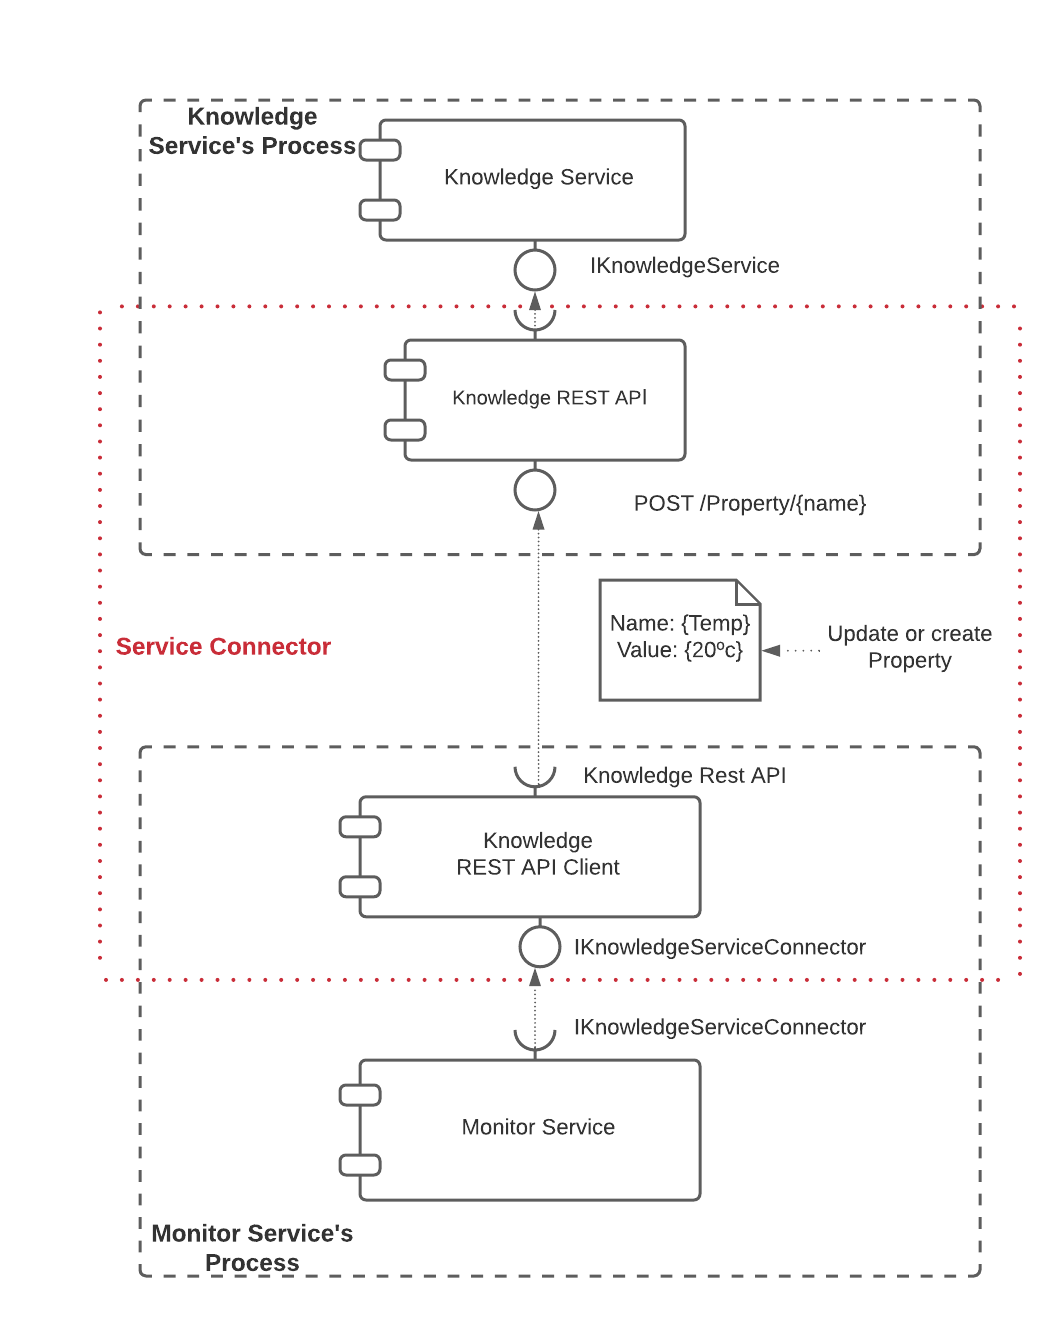
\includegraphics[scale=0.8]{cap_arquitectura/images/Monitor-Knowledge-Connector}
  \caption{Diseño del conector usando implementación Cliente - Servidor}
  \label{fig:monitor-knowledge-connector-architecture}
\end{figure}

\subsection{Notificaciones}

El siguiente mecanismo de comunicación a definir son las notificaciones. Recordemos que esta comunicación es desde un servicio a todos los que se encuentren en la capa superior (\emph{multicast}). No debe estar acoplada a ningún servicio concreto. Potencialmente, todos deberían recibir el mensaje y decidir si procesarlo o no.

Como ejemplo, tomaremos la comunicación entre el servicio de conocimiento y los servicios en la capa superior (el nivel del bucle). Cada vez que se modifique una propiedad o una configuración de un servicio, el servicio emitirá un evento notificando del cambio a la capa superior. Así, por ejemplo, el servicio de análisis sabrá que debe reevaluar las reglas de adaptación.

Sabiendo esto, podemos descartar de entrada GraphQL. Es un protocolo basado en lecturas. Como el objetivo es enviar información a otros servicios, no nos sirve. Respecto a RPC y REST, tampoco nos sirven, no tienen un buen soporte de multicast. Además de que tenemos el requisito de bajo acoplamiento.

Por tanto, optamos por implementarlo usando un \emph{broker} de mensajería. Concretamente, siguiendo el patrón \emph{publish}-\emph{subscribe}. El servicio de conocimiento publicará el evento a través del \emph{broker} de mensajería. Este evento tendrá un \emph{topic} asociado. Todos los servicios interesados deberán suscribirse a este \emph{topic}. El \emph{broker} reenviará el mensaje a una cola específica para cada uno de los servicios suscritos al tema. Así podrán procesarlo cuando puedan, de forma asíncrona.

De esta manera logramos el desacoplamiento de los componentes y permitimos el procesamiento asíncrono de estos eventos.

Aunque potencialmente otros servicios podrían suscribirse a estos cambios, vamos a centrarnos en la suscripción del módulo de análisis.

Los eventos incluirán la información mínima indispensable. En este caso, el nombre de la propiedad que ha cambiado. Esta decisión la tomamos así debido a que es una comunicación asíncrona. Si el evento incluyera el valor de la propiedad y se procesa mucho más tarde, podría derivar en adaptaciones Así evitamos una adaptación incorrecta del sistema. Para evitarlo, incluyendo solo el nombre de la propiedad, obligamos a las reglas a que soliciten el valor de la propiedad en el momento en que se evaluen. Así siempre se ejecutaran con la información actualizada.

El evento que publicaría el módulo de conocimiento cuando cambia una propiedad podría ser como el siguiente (tabla \ref{tab:especificacion-property-changed-integrationevent}):

\newsavebox\propertychangedeventbox
\begin{lrbox}{\propertychangedeventbox}
  \begin{minipage}[t]{2in}
    \begin{verbatim}
{
  "PropertyName":"Temperature"
}
        \end{verbatim}
  \end{minipage}
\end{lrbox}

\begin{table}[htb]
  \centering

  \begin{tabular}{|m{2.3cm}|p{2.5cm}|p{2.6cm}|b{1.5cm}|b{1.5cm}|}
      \hline

      \textbf{Evento} & \multicolumn{2}{|b{0.35\linewidth}|}{\emph{PropertyChangedIntegrationEvent }} & \textbf{\emph{Exchange}} & \emph{AdaptionLoop.Knowledge}  \\
      \hline

      \textbf{Descripción} & \multicolumn{4}{|b{0.6\linewidth}|}{Evento de integración que notifica sobre el cambio de una propiedad adaptación.} \\
      \hline

      \textbf{Propiedades}
            & \emph{propertyName} & \multicolumn{3}{|b{0.6\linewidth}|}{Nombre de la propiedad que ha cambiado.} \\
      \hline

      \textbf{Ejemplo} & \multicolumn{4}{|b{0.7\linewidth}|}{Evento que notifica del cambio de la propiedad \emph{Temperature}:\linebreak
      \usebox\propertychangedeventbox} \\

      \hline
  \end{tabular}

  \caption{Especificación del evento que notifica sobre el cambio de una propiedad del conocimiento.}
  \label{tab:especificacion-property-changed-integrationevent}
\end{table}


Para definir esta comunicación investigamos si había algún estándar equivalente a OpenAPI. Y así es, se llama AsyncAPI\footnote{Página oficial: \url{https://www.asyncapi.com/}}. Es un estándar para especificar la comunicación a través de eventos.Por desgracia, todavía no ha alcanzado el grado de madurez de su homónimo. No tiene el mismo número de herramientas disponible. Por ejemplo, no tiene un catálogo tan amplio de generadores de código que tiene el primero. Tampoco podemos tomar la aproximación de extraer la especificación a partir de una implementación existente.

Aun así, lo utilizaremos para describir nuestros eventos en un formato estándar. En el listing \ref{ls:asyncapi-propertychanged-integrationevent} hemos descrito el mensaje de la tabla \ref{tab:especificacion-property-changed-integrationevent}. Podemos apreciar que es muy parecido a la especificación del método get del listing \ref{ls:openapi-get}.

Aparece la descripción de la estructura del mensaje \texttt{PropertyChangedIntegrationEvent} y su documentación. La mayor diferencia es la mención del canal (el exchange en nuestro caso) y el método (subscribe). Esto indica que los consumidores podrán suscribirse a este evento a partir de este canal.

% TODO: Pintar bien los YAML.
\begin{lstlisting}[language={C++},caption={Ejemplo del evento de integración \emph{builder}.},captionpos=b, label=ls:asyncapi-propertychanged-integrationevent]
asyncapi: 2.4.0
info:
  title: Knowledge Service
  version: 1.0.0
  description: This service contains all the knowledge properties to inform the rest of the loop.
channels:
  AdaptionLoop.Knowledge:
    subscribe:
      message:
        $ref: '#/components/messages/PropertyChangedIntegrationEvent'
components:
  messages:
    PropertyChangedIntegrationEvent:
      description: >-
        Integration event about a change in an adaption property.
      payload:
        type: object
        properties:
          propertyName:
            type: string
            description: The name of the property that changed
\end{lstlisting}

Para implementar este patrón, nuestro conector estará compuesto por tres elementos: un publicador, el \foreign{english}{broker} y un consumidor. El funcionamiento será el siguiente: el servicio de conocimiento recibe una petición para actualizar una propiedad de adaptación. Si esta actualización se lleva a cabo, deberá crear el evento e invocar al publicador, que es un componente que se despliega con este servicio. El publicador recibirá el evento y lo publicará al \foreign{english}{broker} de mensajería en el \foreign{english}{exchange}.

El topic que usaremos es el nombre de la propiedad que ha cambiado.

El broker, que conoce todos los servicios que están subscritos a tema, lo añadirá en la cola de mensajería de cada uno de ellos. Los consumidores, desplegados en cada servicio cliente que se subscribe a estos mensajes, serán notificados de esto. Los procesarán en cuanto puedan. En la \textcolor{red}{figura X} mostramos cómo sería este nuevo conector.

\subsubsection{Peticiones asíncronas}

El último mecanismo de comunicación a diseñar son las \textbf{peticiones asíncronas}. Se trata de aquellas peticiones de trabajo que un microservicio del mismo nivel de la jerarquía le lanza a otro, sin esperar la respuesta. Como comentamos, tenemos dos casos en nuestra arquitectura que requieren de este patrón: la comunicación entre el módulo de análisis y el planificador, y entre el planificador y el ejecutor. Nos centraremos en el primero.

Recordemos que una vez se evalúan las reglas de adaptación, si alguna de ellas se ejecuta, propone un cambio en la configuración del sistema. El módulo de análisis recibirá esta propuesta y se la pasará al planificador. Este generará el plan de adaptación. Esta comunicación se realiza entre servicios en el mismo nivel de la jerarquía.

A la hora de escoger el mecanismo de comunicación, el razonamiento fue muy similar al de las notificaciones. Optamos por implementarlas usando un broker de mensajería, siguiendo el patrón de colas de trabajo. La arquitectura del comunicador es muy similar a la de las notificaciones: un publicador, un broker y un consumidor.

En lugar de ser una comunicación \foreign{english}{fanout} a través de un exchange, como en las notifcaciones, los mensajes van dirigidos a una cola concreta. El servicio consumidor cuenta con una cola de mensajería específica para las peticiones de trabajo. El publicador la conoce y, a través del broker, envía los mensajes allí. EL consumidor los irá recuperando y procesando en cuando esté disponile.

En la tabla \ref{tab:especificacion-system-configuration-change-request-box} presentamos la especificación de la petición asíncrona para solicitar un cambio de configuración de sistema. Vemos que es muy similar a \ref{tab:especificacion-property-changed-integrationevent}.

\newsavebox\systemconfigurationchangerequestbox
\begin{lrbox}{\systemconfigurationchangerequestbox}
  \begin{minipage}[t]{2in}
    \begin{verbatim}
{
  "Timestamp": "2022-06-19T16:38:30.6092751Z",
  "Symptoms":[
    {
      "Name": "temperature-lesser-than-cold-threshold",
      "Value": "true"
    }
  ],
  "ConfigurationRequests":  [
    {
      "ServiceName": "Climatisation.AirConditioner.Service",
      "IsDeployed": true,
      "ConfigurationProperties": [
        {
          "Name": "Mode",
          "Value": "Heating"
        }
      ],
      "Bindings": []
    }
  ]
}
        \end{verbatim}
  \end{minipage}
\end{lrbox}

\begin{table}[htb]
  \centering

  \begin{tabular}{|m{2cm}|m{2.3cm}|m{10cm}|b{0.85cm}|b{2.75cm}|}
      \hline

      \textbf{Nombre} & \multicolumn{2}{|b{0.37\linewidth}|}{\emph{SystemConfigurationChangeRequest}} & \textbf{Cola} & \emph{AdaptionLoop.Planification.Requests}  \\
      \hline

      \textbf{Descripción} & \multicolumn{4}{|b{0.82\linewidth}|}{Petición que representa una propuesta de cambio de la configuración del sistema.} \\
      \hline

      \textbf{Propiedades}
            & \emph{Timestamp} & \multicolumn{3}{|m{0.67\linewidth}|}{Fecha y hora de la petición de cambio.} \\
            \cline{2-5}
            & \emph{Symptoms} & \multicolumn{3}{|m{0.67\linewidth}|}{Colección de síntomas que han desencadenado la petición de cambio.} \\
            \cline{2-5}
            & \emph{Configuration Requests} & \multicolumn{3}{|m{0.67\linewidth}|}{Colección peticiones de configuración de la propuesta de cambio.

            A su vez, está compuesto por:
            \begin{itemize}
              \item \textbf{\emph{ServiceName}}: Identificador del servicio cuya configuración queremos cambiar.
              \item \textbf{\emph{IsDeployed}}: Indica si el servicio debe estar desplegado o no en la siguiente configuración.
              \item \textbf{\emph{Bindings}}: Colección de conexiones que indican a qué servicios debe estar conectado (o no) este servicio en la siguiente configuración.
              \item \textbf{\emph{ConfigurationProperties}}: Colección de pares clave-valor que representan valores de configuración que queremos actualizar.
            \end{itemize}} \\
      \hline

      \textbf{Ejemplo} & \multicolumn{4}{|b{0.82\linewidth}|}{Solicitud de cambio de configuración para cambiar el modo de un aire acondicionado a modo calefacción (\emph{heating}). Fue desencadenada porque la temperatura es menor que un umbral determinado:\linebreak
      \usebox\systemconfigurationchangerequestbox} \\

      \hline
  \end{tabular}

  \caption{Especificación de las peticiones de cambio de configuración del sistema.}
  \label{tab:especificacion-system-configuration-change-request-box}
\end{table}

Respecto a la especificación con AsyncAPI, las peticiones asíncronas no están soportadas todavía. El grupo está todavía estudiando cómo implementarlas. \footnotetext{Discusión disponible en: \url{https://github.com/asyncapi/spec/pull/594}}. Está propuesta para incluirla en la versión 3.0.0 de la especificación. Como mencionamos anteriormente, el estándar todavía es muy joven y tiene trabajo por delante.

En cuanto a sus componentes, el conector seguiría la siguiente arquitectura: \textcolor{red}{dibujo de arquitectura}.

\subsubsection{Diseño final}

Añadir diagrama con el diseño final, mostrando el diseño de los componentes con todos los conectores.



\chapter{Implementación}
\label{chap:implementación}

Uno de los objetivos de este trabajo era verificar que la nueva arquitectura fuera viable. La mejor forma de hacerlo es aplicarla en la práctica. En un primer momento consideramos refactorizar el bucle MAPE-K \foreign{english}{Lite} para realizar estas pruebas. Pero, debido a su complejidad y las restricciones de tiempo, optamos por implementar una versión reducida del mismo.

Este prototipo se desarrolló a partir de la especificación del sistema existente. Esto nos permitió definir las nuevas APIs de comunicación e implementar la funcionalidad básica. Gracias a él, pudimos evolucionar el diseño según detectábamos nuevas necesidades o problemas que no resolvía nuestra arquitectura. Cuando llegue el momento de la refactorización del bucle original, podremos emplear las APIs desarrolladas.

En este capítulo nos centraremos en la implementación de los microservicios del nivel del bucle y del conocimiento. Dejaremos para más adelante, en el capítulo \ref{chap:caso_estudio} - \nameref{chap:caso_estudio}, la descripción de la implementación del recurso manejado. En este capítulo nos centraremos más en la implementación y en las tecnologías empleadas. En el otro, describiremos mediante un caso de estudio cómo encajan los componentes y cómo opera el sistema completo.

La implementación se llevó a cabo en 4 hitos distintos:

\section{Servicio de monitorización y conocimiento}

En esta primera etapa se desarrolló el proceso de monitorización. Este abarca desde que una sonda realiza sus mediciones hasta que se graban en el conocimiento. Esto implicó implementar varios componentes: las sondas y monitores del caso de estudio (capítulo \ref{chap:caso_estudio}), el componente de monitorización del bucle MAPE-K y la base de conocimiento (figura \ref{fig:hito-1-monitorizacion}).

\begin{wrapfigure}{r}{0.16\linewidth}
  \vspace{-15pt}
  
\includegraphics[scale=0.15]{cap_implementacion/images/dotnet-logo}
  \centering
\end{wrapfigure}

Para su desarrollo se optó por el lenguaje C\# y el \foreign{english}{framework} ASP.NET\footnote{Página oficial: \url{https://docs.microsoft.com/en-us/aspnet/core/introduction-to-aspnet-core}}. Este \emph{framework} es específico para implementar servidores web. Forma parte de la plataforma .NET de Microsoft. Lo elegimos por nuestra experiencia de desarrollo en ella. Además de que soporta los principales sistemas operativos (Windows, Linux y Mac).

\begin{figure}[h!]
  \centering
  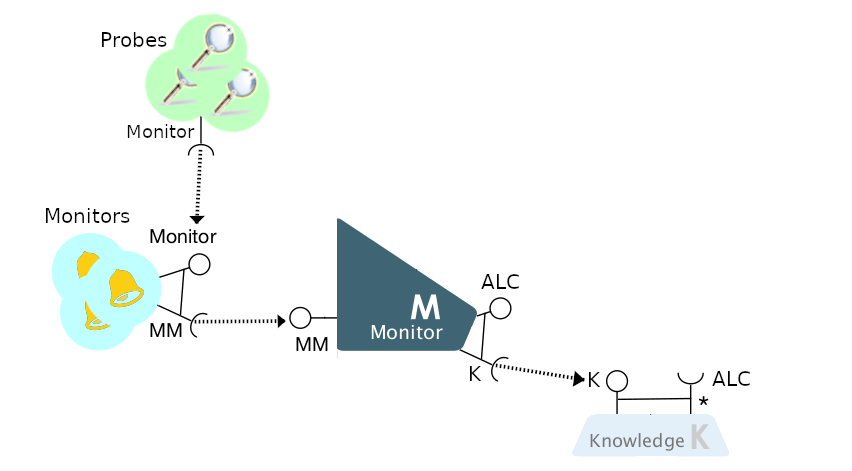
\includegraphics[scale=0.45]{cap_implementacion/images/hito-1-monitorizacion}
  \caption{Componentes desarrollados durante el primer hito: Sondas, monitores, el módulo de monitorización y el conocimiento.}
  \label{fig:hito-1-monitorizacion}
\end{figure}

\subsection{Peticiones síncronas}

En este hito se prototiparon las peticiones síncronas (flechas negras de la figura \ref{fig:hito-1-monitorizacion}). Los servicios que las implementan exponen APIs REST mediante \foreign{english}{endpoints} HTTP. Por ejemplo, el servicio de conocimiento expone operaciones que permiten recuperar o modificar propiedades de adaptación. Nos centraremos en la primera, ya descrita en la tabla \ref{tab:especificacion-get-property}.

En el fragmento \ref{ls:csharp-get} mostramos su implementación. Podemos observar que se trata de un método llamado \emph{GetProperty}. Su lógica es sencilla: busca en un diccionario la propiedad cuyo nombre recibe por parámetro. Si la encuentra, devuelve su valor con un código HTTP (\texttt{200 OK}). En caso contrario, sólo devuelve un código de error que describe el motivo de fallo: formato de la petición incorrecto (\texttt{400 - Bad Request}) o que no se ha encontrado la propiedad (\texttt{404 - Not Found}).

Se puede comprobar que el método cuenta con una serie de comentarios (líneas \texttt{1-8}) y atributos (\texttt{10-12}). En conjunto estos conforman su documentación. Describen qué hace el método, sus parámetros de entrada y posibles respuestas. OpenAPI puede aprovecharlos para generar una especificación más completa. Resulta entonces muy recomendable incluirlos.

\begin{lstlisting}[ caption={Implementación del método \texttt{GetProperty} decorado para generar la especificación OpenAPI.\protect\footnotemark},captionpos=b, label=ls:csharp-get]
  /// <summary>
  ///    Gets a property given its name.
  /// </summary>
  /// <param name="propertyName"> The name of the property to find. </param>
  /// <returns> An IActionResult with result of the query. </returns>
  /// <response code="200"> The property was found. Returns the value of the property. </response>
  /// <response code="404"> The property was not found. </response>
  /// <response code="400"> There was an error with the provided arguments. </response>
  [HttpGet("{propertyName}")]
  [ProducesResponseType(typeof(PropertyDTO), StatusCodes.Status200OK)]
  [ProducesResponseType(StatusCodes.Status404NotFound)]
  [ProducesResponseType(StatusCodes.Status400BadRequest)]
  public IActionResult GetProperty([FromRoute]string propertyName)
  {
      if (string.IsNullOrEmpty(propertyName))
      {
          return BadRequest();
      }

      bool propertyFound =
          properties.TryGetValue(propertyName, out PropertyDTO property);

      if (!propertyFound)
      {
          return NotFound();
      }

      return Ok(property);
  }
\end{lstlisting}

\footnotetext{Código disponible \href{https://github.com/Starkie/TFM-DistributedAutoadaptiveSystems/blob/1db95346290cb55edbfd5efb717785bcd06def79/src/AutoAdaptativeSystem/AdaptionLoop/Knowledge/Controllers/PropertyController.cs\#L44-L77}{aquí}.}

Para generar la especificación empleamos la librería \emph{Swashbuckle.AspNetCore}\footnote{Página oficial: \url{https://github.com/domaindrivendev/Swashbuckle.AspNetCore}}. Esta es capaz de extraerla de un servicio ASP.NET existente. En el fragmento \ref{ls:openapi-get}, se muestra cómo se describe el \foreign{english}{endpoint} en este estándar. Podemos confirmar que se han incluido los comentarios y atributos que documentaban en el código. Por ejemplo, figuran los parámetros, las respuestas y sus códigos HTTP, etc. Es destacable la similitud que presenta con la especificación de la tabla \ref{tab:especificacion-get-property}.

\begin{lstlisting}[style=json,caption={Especificación OpenAPI del método para obtener una propiedad del conocimiento (\lstinline{GetProperty}). \protect\footnotemark},captionpos=b, label=ls:openapi-get]
"paths": {
  "/Property/{propertyName}": {
    "get": {
      "tags": [
        "Property"
      ],
      "summary": "Gets a property given its name.",
      "parameters": [{
          "name": "propertyName",
          "in": "path",
          "description": "The name of the property to find.",
          "required": true,
          "schema": {
            "type": "string"
          }
        }
      ],
      "responses": {
        "200": {
          "description": "The property was found. Returns the value of the property.",
          "content": {
            "application/json": {
              "schema": {
                "$ref": "#/components/schemas/PropertyDTO"
              }
            }
          }
        },
        "404": { "description": "The property was not found.", },
        "400": {
          "description": "There was an error with the provided arguments.",
        }
      }
    }
  }
\end{lstlisting}

\footnotetext{Código disponible \href{https://github.com/Starkie/TFM-DistributedAutoadaptiveSystems/blob/1db95346290cb55edbfd5efb717785bcd06def79/src/AutoAdaptativeSystem/AdaptionLoop/Knowledge/Knowledge.Service-OpenAPISpec.json\#L108-L187}{aquí}.}

A partir de la especificación, esta librería añade al servicio una interfaz de usuario. Esta es accesible a través del \foreign{english}{endpoint} \texttt{/swagger}. Allí, se nos servirá una página web con el listado de todas las operaciones que ofrece el servicio (figura \ref{fig:swagger-knowledge-ui}). De cada una nos muestra su documentación, sus parámetros, etc. Incluso permite ejecutarlas. Así, puede ser de ayuda a los desarrolladores que necesiten trabajar con esta API.

\begin{figure}[htb]
  \centering
  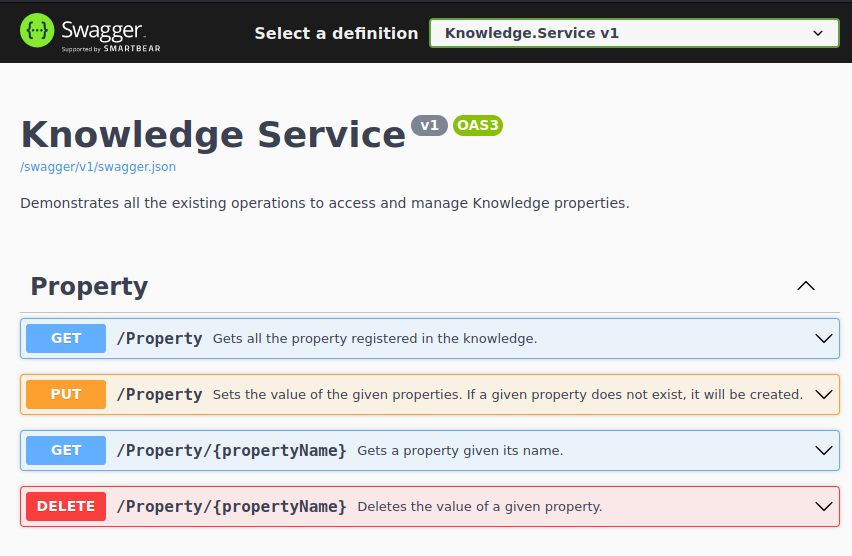
\includegraphics[scale=1.5]{cap_implementacion/images/swagger-knowledge-ui}
  \caption{Interfaz de usuario ofrecida por Swagger para el servicio de conocimiento. Se genera a partir de la especificación OpenAPI.}
  \label{fig:swagger-knowledge-ui}
\end{figure}

Por otro lado, también se pudo generar el API \foreign{english}{client}. Como comentamos en la sección \ref{chap:OpenAPI} - \nameref{chap:OpenAPI}, tenemos gran variedad de generadores de código a nuestra disposición. Nosotros optamos por la librería \texttt{OpenAPI.Generator}\footnote{Página del proyecto: \url{https://github.com/OpenAPITools/openapi-generator}}. En concreto, por un generador de código de \verb|C#|. Usándolo, pudimos obtener una librería que permite contactar con el servicio, sin necesidad de implementar mucho código. Por ejemplo, el componente de monitorización del bucle contacta con el conocimiento a través de un API \foreign{english}{client}.

Además, podremos utilizar estas herramientas durante la refactorización del bucle MAPE-K original. Aunque este está desarrollado en Java, podremos generar el código a partir de la especificación de nuestra implementación. Tanto de los clientes como los servidores. Esto ayudará a agilizar enormemente el proceso de desarrollo.

\subsection{Componentes: Módulos de monitorización y conocimiento}

Los componentes implementados en este hito son muy sencillos. Simplemente validan las mediciones de las sondas y extraen de ellas las propiedades de adaptación. Ya hemos hablado de la implementación del servicio de conocimiento. Este ofrece simplemente operaciones de lectura y escritura sobre las propiedades de adaptación y las claves de configuración de los recursos manejados.

Por encima de este, tenemos al servicio de monitorización. En nuestra implementación, actúa como intermediario entre los monitores de la solución y el conocimiento. Ofrece \foreign{english}{endpoints} útiles para los monitores, como puede ser reportar sus mediciones o la lectura del conocimiento. De esta forma, los monitores de solución podrán informarse para determinar si una medición es válida o no. Para conectar todos estos servicios se emplearon las peticiones síncronas, que describiremos anteriormente.

\section{Servicio de análisis y reglas}
\label{sec:implementacion-modulo-reglas}

La siguiente etapa que desarrollamos fue la evaluación de las reglas de adaptación. Esta requería implementar el servicio de análisis del bucle MAPE-K y los servicios de reglas de la solución. También necesitamos el mecanismo de las comunicaciones ascendentes: las notificaciones. Con ellas evitamos que los componentes se acoplaran a los de la capa superior.

\subsection{Notificaciones}

\begin{wrapfigure}{r}{0.13\linewidth}
  \vspace{-10pt}
  
\includegraphics[scale=0.09]{cap_implementacion/images/rabbitmq}
  \centering
  \vspace{-10pt}
\end{wrapfigure}

Comenzaremos describiendo el desarrollo de las notificaciones (flechas moradas de la figura \ref{fig:hito-2-analisis}). Como ya se describió en la sección \ref{sec:notificaciones}, este mecanismo se implementó mediante un \foreign{english}{broker} de mensajería. Se elegió \texttt{RabbitMQ}\footnote{Página oficial: \url{https://www.rabbitmq.com/}} para el proyecto, un \foreign{english}{broker} sencillo y ampliamente utilizado. \cite{newmanBuildingMicroservicesDesigning2021}

Para implementar los publicadores y consumidores de nuestro conector, utilizamos una librería llamada \texttt{Rebus}\footnote{Página oficial: \url{https://github.com/rebus-org/Rebus}}. Esta nos permitía interactuar con el bus abstrayéndonos de su tecnología concreta. Así, podríamos cambiar de tecnología de transporte en cualquier momento sin tener que modificar nuestros servicios.

Finalmente, para desacoplar la funcionalidad del servicio de la publicación y consumición de mensajes del bus, empleamos \texttt{MediatR}\footnote{Página oficial: \url{https://github.com/jbogard/MediatR}}. Esta librería implementa el patrón mediador\footnote{Patrón mediador: \url{https://refactoring.guru/design-patterns/mediator}}. Permite propagar mensajes dentro de un mismo proceso, sin necesidad de que el emisor ni el receptor se referencien. Para ello, se definen uno o más manejadores (\foreign{english}{handlers}) que capturan y procesan el mensaje. En el caso de las notificaciones propagaremos eventos de integración.

Para describir la implementación nos centraremos en la comunicación entre el módulo de conocimiento y el servicio de análisis. Una vez se confirma la escritura de una propiedad de adaptación en el conocimiento, este debe notificar a los servicios en la capa superior. Para ello, comienza propagando internamente un \textbf{evento de integración} usando el mediador (línea 11 del fragmento \ref{ls:knowledge-set-property}).

\begin{lstlisting}[caption={Implementación del método que asigna valor a una propiedad. Muestra un ejemplo de propagación interna de eventos de integración.\protect\footnotemark},captionpos=b, label=ls:knowledge-set-property]
private async Task SetProperty(SetPropertyDTO propertyDto)
{
    var newValue = new()
    {
        Value = propertyDto.Value,
        LastModification = DateTime.UtcNow,
    };

    properties.AddOrUpdate(propertyDto.Name, newValue, (_, _) => newValue);

    await _mediator.Send(
      new PropertyChangedIntegrationEvent(propertyDto.Name));
}

\end{lstlisting}

\footnotetext{Código disponible \href{https://github.com/Starkie/TFM-DistributedAutoadaptiveSystems/blob/1db95346290cb55edbfd5efb717785bcd06def79/src/AutoAdaptativeSystem/AdaptionLoop/Knowledge/Controllers/PropertyController.cs\#L106-L119}{aquí}.}

El mediador determina que el componente publicador es el destinatario de este evento y lo invoca. Para detectarlo, se basa en las interfaces que implementa (línea 2 del fragmento \ref{ls:knowledge-property-changed-publisher}). Este componente publica el evento en el bus de mensajería (línea 15). Rebus, en base a la configuración del servicio, lo enviará a nuestra instancia de \texttt{RabbitMQ}. Todos los suscriptores de este evento recibirán el mensaje en su cola.

\begin{lstlisting}[caption={El publicador de eventos captura el evento de integración y lo publica en el bus.\protect\footnotemark},captionpos=b, label=ls:knowledge-property-changed-publisher]
public class PropertyChangedIntegrationEventPublisher
  : IIntegrationEventPublisher<PropertyChangedIntegrationEvent>
{
  private readonly IBus _bus;

  public PropertyChangedIntegrationEventPublisher(IBus bus)
  {
      _bus = bus;
  }

  public async Task<Unit> Handle(
      PropertyChangedIntegrationEvent notification,
      CancellationToken cancellationToken)
  {
      await _bus.Publish(notification);

      return Unit.Value;
  }
}
\end{lstlisting}

\footnotetext{Código disponible \href{https://github.com/Starkie/TFM-DistributedAutoadaptiveSystems/blob/1db95346290cb55edbfd5efb717785bcd06def79/src/AutoAdaptativeSystem/AdaptionLoop/Knowledge/EventHandlers/PropertyChangedIntegrationEventPublisher.cs}{aquí}.}

Finalmente, en el servicio de análisis, se encuentra el componente consumidor (fragmento \ref{ls:analysis-property-changed-consumer}). \texttt{Rebus} obtiene el evento de la cola de mensajería y se lo transmite. Este lo recibe y lo propaga internamente en el servicio (línea 20). Todos los \foreign{english}{handlers} del evento lo recibirán y podrán tratarlo. En este caso, las reglas de adaptación.

\begin{lstlisting}[caption={El consumidor recibe el evento de integración del bus y lo propaga internamente. Todos los \foreign{english}{handlers} de este evento lo recibirán.\protect\footnotemark},captionpos=b, label=ls:analysis-property-changed-consumer]
public class PropertyChangedIntegrationEventConsumer
  : IIntegrationEventConsumer<PropertyChangedIntegrationEvent>
{
  private readonly IMediator _mediator;

  public PropertyChangedIntegrationEventConsumer(IMediator mediator)
  {
      _mediator = mediator;
  }

  public async Task Handle(PropertyChangedIntegrationEvent message)
  {
      await _mediator.Publish(message);
  }
}
\end{lstlisting}

\footnotetext{Código disponible \href{https://github.com/Starkie/TFM-DistributedAutoadaptiveSystems/blob/1db95346290cb55edbfd5efb717785bcd06def79/src/AutoAdaptativeSystem/AdaptionLoop/Analysis/Application/Properties/Events/PropertyChangedIntegrationEventConsumer.cs}{aquí}.}

\subsection{Componentes: Servicio de análisis y módulos de reglas}

En este hito se desarrollaron los servicios de análisis y de los módulos de reglas (figura \ref{fig:hito-2-analisis}). En cuanto al del módulo de análisis, este realmente no cuenta con mucha lógica. Participa como intermediario entre el conocimiento y los servicios de reglas. Como hemos visto, recibe los eventos de cambios en las propiedades y los propaga a la capa superior. Ofrece operaciones de solo lectura del conocimiento. Así, impedimos las escrituras por parte de las reglas.

\begin{wrapfigure}{l}{0.3\linewidth}
  \vspace{-20pt}
  \centering
  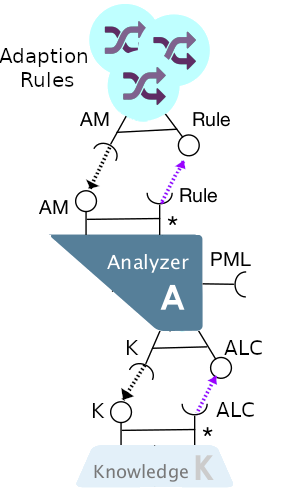
\includegraphics[scale=0.6]{cap_implementacion/images/hito-2-analisis}
\caption{Segundo hito: reglas de adaptación y módulo de análisis.}
  \label{fig:hito-2-analisis}
  \vspace{-10pt}
\end{wrapfigure}

Más tarde nos dimos cuenta que se podría considerar como un servicio ''anémico''\footnote{Similar a los objetos anémicos, sin apenas lógica: \url{https://www.martinfowler.com/bliki/AnemicDomainModel.html}}. \cite{singjaiPatternsDerivingAPIs2021} No tiene apenas lógica propia. Cuando se realice la refactorización del bucle original, se podría evaluar si tiene sentido mantener esta división. Si no es así, debería desplegarse como una librería que consuman todos los servicios de reglas de adaptación. En trabajos posteriores, este servicio podría ampliarse añadiendo autenticación y autorización. Así, se podría evitar que servicios no autorizados accedan a sus operaciones o soliciten adaptaciones maliciosas.

Respecto a los módulos de reglas, a continuación ofrecemos una implementación de referencia. En el fragmento \ref{ls:adaption-rule-base} mostramos la clase base de las reglas de adaptación. Se desarrolló siguiendo el patrón plantilla (o \foreign{english}{template})\footnote{\url{https://refactoring.guru/design-patterns/template-method}}. Define un método que evalúa la condición de la regla (\texttt{EvaluateCondition}) y, si esta se cumple, la ejecuta (\texttt{Execute}). Aquellas reglas que hereden de esta deberán de implementar ambos métodos.

Vemos además que está suscrita a los eventos de integración de cambio de propiedad de adaptación y cambio en la configuración del sistema (líneas 2-3). Cuando el consumidor reciba uno de ellos, lo propagará internamente. Todas las reglas afectadas lo capturarán y se evaluarán.

\begin{lstlisting}[caption={Clase base para implementar reglas de adaptación. Se evalúa la condición, y si esta se cumple, se ejecuta. \protect\footnotemark},captionpos=b, label=ls:adaption-rule-base]
public abstract class AdaptionRuleBase
    : IIntegrationEventHandler<PropertyChangedIntegrationEvent>,
      IIntegrationEventHandler<ConfigurationChangedIntegrationEvent>
{
    // ..
    private async Task Handle()
    {
        try
        {
            if (await EvaluateCondition())
            {
                await Execute();
            }
        }
        catch (Exception e)
        {
            _diagnostics.RuleEvaluationError(_ruleName, e);

            throw;
        }
    }

    protected abstract Task<bool> EvaluateCondition();

    protected abstract Task Execute();
}
\end{lstlisting}

\footnotetext{Código disponible \href{https://github.com/Starkie/TFM-DistributedAutoadaptiveSystems/blob/1db95346290cb55edbfd5efb717785bcd06def79/src/AutoAdaptativeSystem/Climatisation/Rules/EventHandlers/Rules/AdaptionRuleBase.cs}{aquí}.}

Las reglas deben indicar de qué propiedades o claves de configuración dependen. Para ello, hemos implementado una serie de atributos que decoran sus clases. En el fragmento \ref{ls:adaption-rule-dependencies} mostramos un ejemplo. En la línea 1 tenemos el atributo que describe las dependencias con la propiedad de adaptación \texttt{Temperature}. Por otro lado, en las líneas 2-5 tenemos la declaración de dependencias con dos claves de configuración del servicio \texttt{Climatisation.AirConditioner}: \texttt{TargetTemperature} y \texttt{Mode}.

\begin{lstlisting}[caption={Las reglas declaran sus dependencias sobre propiedades de adaptación usando atributos. Estos se utilizarán para las suscripciones a los temas de los eventos.\protect\footnotemark},captionpos=b, label=ls:adaption-rule-dependencies]
[RuleKnowledgePropertyDependency(ClimatisationConstants.Property.Temperature)]
[RuleServiceConfigurationDependency(
    ClimatisationAirConditionerConstants.AppName,
    ClimatisationAirConditionerConstants.Configuration.TargetTemperature,
    ClimatisationAirConditionerConstants.Configuration.Mode)]
public class DisableAirConditionerWhenCoolingAndTargetTemperatureAchievedAdaptionRule
  : AdaptionRuleBase
{
    // ...
}
\end{lstlisting}

\footnotetext{Código disponible \href{https://github.com/Starkie/TFM-DistributedAutoadaptiveSystems/blob/1db95346290cb55edbfd5efb717785bcd06def79/src/AutoAdaptativeSystem/Climatisation/Rules/EventHandlers/Rules/DisableAirConditionerWhenCoolingModeEnabledAndTargetTemperatureAchievedRule.cs\#L14-L19}{aquí}.}

En base a los atributos, el servicio se suscribirá a los \foreign{english}{topics} de las notificaciones que emite el módulo de análisis. Para leerlos emplearemos la \textbf{reflexión}: analizaremos el ensamblado buscando las reglas y obtendremos los valores de sus atributos. Se le pasarán a \texttt{Rebus}, que gestionará la suscripción con \texttt{RabbitMQ}.

\section{Servicio de planificación y peticiones de cambio}

En el tercer hito se implementaron las peticiones de cambio en la configuración del sistema. Este proceso comienza con la ejecución del cuerpo de las reglas y acaba con la generación de un \textbf{plan de cambio}. Esto requirió del desarrollo de un nuevo servicio: el planificador (figura \ref{fig:hito-3-planificador}). En este hito también surgió la necesidad de las peticiones asíncronas, el tercer protocolo de comunicación.

\begin{figure}[h!]
  \centering
  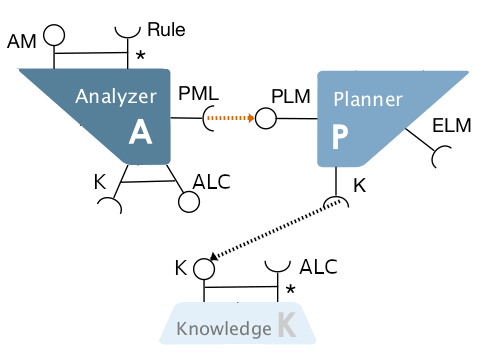
\includegraphics[scale=0.50]{cap_implementacion/images/hito-3-planificador}
  \caption{Componente desarrollado durante el tercer hito: Planificador.}
  \label{fig:hito-3-planificador}
\end{figure}

\subsection{Peticiones asíncronas}

Las peticiones asíncronas son el tercer mecanismo de comunicación de nuestra arquitectura (flecha naranja en la figura \ref{fig:hito-3-planificador}). Estas permiten interactuar a los servicios que pertenecen a una misma capa. Para describir su implementación tomaremos de ejemplo las peticiones de cambio de las reglas de adaptación.

Cuando la regla evalúa su condición y estima que es necesaria una acción correctiva, se ejecuta su método \texttt{Execute}. Este método envía una petición que describe cuál debería ser el siguiente estado del recurso manejado. Por ejemplo, qué componentes deben estar presentes o no, qué conexiones deben existir, etc.

Las reglas comunicarán esta solicitud al módulo de análisis mediante una petición síncrona. Para simplificar el proceso, desarrollamos un \foreign{english}{builder}\footnote{Patrón \foreign{english}{builder}: \url{https://refactoring.guru/design-patterns/builder}} de peticiones por encima de su API \foreign{english}{client}. En el fragmento \ref{ls:change-request-builder} mostramos un ejemplo. Allí se indica cuál debería ser la siguiente configuración para el servicio \texttt{Climatisation AirConditioner Service} (líneas 7-14). Deberá estar activo (línea 10) y su propiedad \texttt{Mode} deberá tener el valor \texttt{Cooling} (líneas 11-13). También se incluye el síntoma que desencadena el cambio (línea 6).

\begin{lstlisting}[caption={Implementación de la misma petición siguiendo el patrón \emph{builder}.\protect\footnotemark},captionpos=b, label=ls:change-request-builder]
protected override async Task Execute()
{
  await _systemService.RequestConfigurationChange(changeRequest =>
  {
    changeRequest
      .ForSymptom(TemperatureGreaterThanHotThreshold)
      .WithService(ClimatisationAirConditionerConstants.AppName, service =>
      {
        service
          .MustBePresent()
          .WithParameter(
            ClimatisationAirConditionerConstants.Configuration.Mode,
            AirConditioningMode.Cooling.ToString());
      });
  });
}
\end{lstlisting}

\footnotetext{Código disponible \href{https://github.com/Starkie/TFM-DistributedAutoadaptiveSystems/blob/1db95346290cb55edbfd5efb717785bcd06def79/src/AutoAdaptativeSystem/Climatisation/Rules/EventHandlers/Rules/DisableAirConditionerWhenCoolingModeEnabledAndTargetTemperatureAchievedRule.cs\#L74-L88}{aquí}.}

El servicio de análisis recibirá la petición y la redirigirá al planificador mediante una petición asíncrona. Su implementación es muy similar a la de las notificaciones, explicada en detalle en el apartado anterior. La mayor diferencia radica en la cardinalidad de la comunicación: en lugar de publicarlo en un \foreign{english}{exchange}, el mensaje se publicará directamente en la cola de trabajo. Sólo lo debería procesará un servicio.

Como la comunicación es tan similar, únicamente cambiará la implementación del publicador. La mayor diferencia se puede apreciar en el fragmento \ref{ls:request-publisher}. Allí, vemos que el mensaje se enruta directamente a la cola \texttt{PlanningServiceQueue} (línea 15). También cambiarán las interfaces que deban implementar los componentes. En este caso \texttt{IRequestPublisher} en lugar de \texttt{IIntegrationEventPublisher} (línea 2).

\begin{lstlisting}[caption={Las peticiones asíncronas se publican a una cola determinada.\protect\footnotemark},captionpos=b, label=ls:request-publisher]
public class SystemConfigurationChangeRequestPublisher
  : IRequestPublisher<SystemConfigurationChangeRequest>
  where TRequest : Request
{
  public SystemConfigurationChangeRequestPublisher(IBus bus)
  {
      _bus = bus;
  }

  public async Task<Unit> Handle(
      SystemConfigurationChangeRequest request,
      CancellationToken cancellationToken)
  {
      await _bus.Advanced.Routing.Send(
          AdaptionLoopPlanningConstants.Queues.PlanningServiceQueue,
          request);

      return Unit.Value;
  }
}
\end{lstlisting}

\footnotetext{Código disponible \href{https://github.com/Starkie/TFM-DistributedAutoadaptiveSystems/blob/1db95346290cb55edbfd5efb717785bcd06def79/src/AutoAdaptativeSystem/AdaptionLoop/Analysis/Application/SystemConfiguration/Requests/SystemConfigurationChangeRequestIntegrationEventPublisher.cs}{aquí}.}

\subsection{Componentes: Servicio de planificación}

El planificador consumirá esta petición de cambio y deberá elaborar un \textbf{plan de adaptación}. Para ello, deberá determinar qué acciones son necesarias para alcanzar el estado deseado. Lo comparará con el estado actual, almacenado en el conocimiento, y añadirá al plan las \textbf{acciones de adaptación} requeridas. Si el sistema ya estuviera en ese estado, el plan de cambio se quedará vacío y no se propagará.

Por ejemplo, en el fragmento \ref{ls:adaption-change-plan} encontramos un plan de adaptación para la regla descrita en la sección anterior. Solo contiene una acción de adaptación: cambiar el valor de la propiedad \texttt{Mode} a \texttt{Cooling}. Como el servicio de aire acondicionado ya estaba en funcionamiento, no se ha incluido una acción para desplegarlo.

\begin{lstlisting}[style=json,caption={Plan de adaptación generado para la regla anterior. Solo contiene una acción de adaptación: cambiar la configuración \texttt{Mode} del servicio \texttt{AirConditioner}.},captionpos=b, label=ls:adaption-change-plan]
{
  "ChangePlan": {
    "Timestamp": "2022-07-09T09:53:01.1868834Z",
    "Actions":
    [
      {
        "Type": "SetParameter",
        "ServiceName": "Climatisation.AirConditioner.Service",
        "PropertyName": "Mode",
        "PropertyValue": "Cooling"
      }
    ]
  },
  "Symptoms":
  [
    {
      "Name": "temperature-lesser-than-cold-threshold",
      "Value": "true"
    }
  ]
}
\end{lstlisting}

Para reducir el alcance del proyecto, no validaremos la viabilidad del plan de adaptación. Se descartó implementar los planificadores específicos de la solución.  Sólo contaremos con la estrategia por defecto: validar que el plan contenga al menos una acción.

\section{Servicio de ejecución y efectores}


En el hito final desarrollamos la ejecución del plan de adaptación. Cerramos así el ciclo del bucle de adaptación. Esto requirió del módulo ejecutor, los ejecutores de la solución y los efectores del recurso manejado (figura \ref{fig:hito-4-ejecutor}).

\begin{figure}[h!]
  \centering
  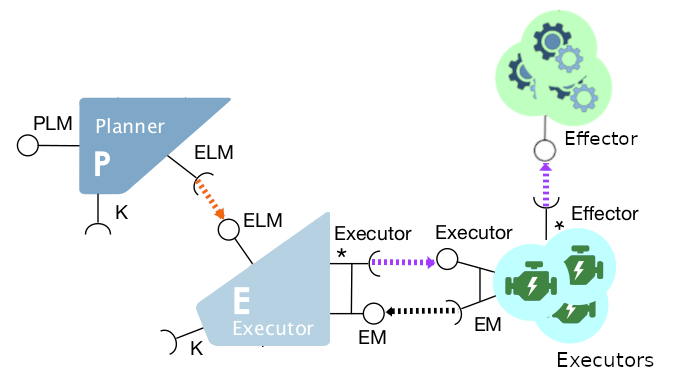
\includegraphics[scale=0.55]{cap_implementacion/images/hito-4-ejecutor}
  \caption{Componentes desarrollados durante el cuarto hito: Módulo de ejecución, ejecutores y efectores.}
  \label{fig:hito-4-ejecutor}
\end{figure}

\subsection{Componentes: Servicio de ejecución, ejecutores y efectores}

El servicio de ejecución recibe el plan de adaptación del planificador mediante una petición asíncrona. Para ejecutarlo, deberá agrupar las acciones por el servicio afectado y distribuirlas entre los distintos ejecutores de la solución. Para transmitirlas, enviará cada grupo de acciones mediante una notificación. Pueden existir varios ejecutores en una misma solución y no deberíamos acoplarnos a ellos. El evento enviado es muy similar al que ya mostramos en el fragmento \ref{ls:adaption-change-plan}.

Cuando un ejecutor capture esta notificación, procesará las acciones asignadas. Este componente será el encargado de traducir las acciones de adaptación a manipulaciones de efectores del recurso manejado. Dependiendo del tipo de acción, el efector hará una acción u otra: desplegar un servicio, o eliminarlo, cambiar la configuración, etc. Para reducir el alcance del proyecto, sólo implementamos las adaptaciones de tipo \foreign{english}{set parameter}.

En cuanto a la comunicación con el efector, este caso es un tanto especial. El mecanismo dependerá del sistema manejado; de si tenemos control sobre su implementación. Si no es así, tendremos que adaptarnos a aquellos protocolos que ofrezca el recurso (HTTP, mensajería...).

Continuando con el ejemplo del aire acondicionado, el ejecutor recibiría la notificación con las acciones a ejecutar. En este caso, cambiar el modo de funcionamiento a enfriar. Para ello, enviará la acción al efector y se ejecutará. Una vez se confirme el cambio, una sonda lo detectará y notificará a su monitor. Se seguirá el mismo proceso que con las demás mediciones para guardarlo en la base de conocimiento.


\chapter{Caso de estudio: Sistema de climatización}
\label{chap:caso_estudio}

Para verificar la arquitectura definida, decidimos implementar un pequeño sistema autoadaptativo. Se trata de un sistema de climatización, que gestiona la temperatura de una habitación. Para ello, dispondremos de un aire acondicionado, que calentará o enfriará la habitación según corresponda.

\section{Análisis}

El primer paso es capturar los requisitos del sistema a implementar. Cómo hemos comentado, queremos desarrollar un sistema de climatización. Este sistema regulará la temperatura de una habitación mediante el uso de un aparato de aire acondicionado.

El aparato de aire acondicionado ofrece tres modos de funcionamiento: un modo para calentar la estancia, otro para enfriarla, y un estado neutral (apagado). Además, lo hemos dotado con un termómetro interno que nos reporta la temperatura periódicamente.

Para poder climatizar la habitación, necesitamos que el usuario defina su temperatura objetivo: la temperatura de confort. Cambios en la temperatura deberán activar o desactivar el aparato para mantenerla.

Además, nos interesa evitar que el aire acondicionado se encienda y se apague constantemente cuando se alcance o sobrepase esta temperatura. Por ello, definimos unas temperaturas umbrales, tanto de frío como de calor, a partir de las cuales se encenderá el aparato.

\section{Diseño}

Del análisis anterior ya podemos deducir la existencia de dos componentes: un aparato de aire acondicionado (el sistema gestionado) y un termómetro (la sonda). Aparte de ellos, deberemos implementar la infraestructura necesaria para comunicarse con nuestro bucle MAPE-K: monitores, módulos de reglas y efectores que nos permitan interactuar con el sistema manejado.

Para describir el diseño usaremos la notación de sistemas autoadaptativos descrita en \cite{fonsEspecificacionSistemasAutoadaptativos2021}.

\subsection{Sondas:}

Para implementar el sistema, requerimos de las siguientes sondas:

\begin{longtable}{|r p{11.5cm}|}
    \hline
    \textbf{Sonda:} & \emph{thermometer}  \\
    \textbf{Descripción:} & Reporta la temperatura actual de la habitación (en ºc). \\
    \textbf{Monitor:} & \emph{Climatisation.Monitor} \\
    \textbf{Datos:} & \emph{temperature} \\
    \hline
    \textbf{Sonda:} & \emph{airconditioner-mode-changed-probe}  \\
    \textbf{Descripción:} & Reporta el modo de funcionamiento del aire acondicionado cuando este cambia. \\
    \textbf{Monitor:} & \emph{Climatisation.Monitor} \\
    \textbf{Datos:} & \emph{airconditioner-mode} \\
    \hline
    \textbf{Sonda:} & \emph{airconditioner-adaption-loop-registration}  \\
    \textbf{Descripción:} & Cuando arranca el servicio de aire acondicionado, registra la configuración inicial del sistema. \\
    \textbf{Monitor:} & \emph{Climatisation.Monitor} \\
    \textbf{Datos:} & \emph{airconditioner.is-deployed}, \emph{airconditioner-mode}, \emph{target-temperature}, \emph{cold-temperature-threshold}, \emph{hot-temperature-threshold} \\
    \hline

    \caption{Sondas del sistema de climatización.}
    \label{tab:climatisation-probes}
\end{longtable}

\subsection{Propiedades de adaptación:}

También podemos deducir cuáles son nuestras propiedades de adaptación:

\begin{longtable}{|r p{11.5cm}|}
    \hline
    \textbf{Propiedad:} & \emph{temperature}  \\
    \textbf{Descripción:} & Representa la temperatura actual de la habitación (en ºC).  \\
    \textbf{Tipo de dato:} & \emph{float} \\
    \hline
    \textbf{Propiedad:} & \emph{target-temperature}  \\
    \textbf{Descripción:} & La temperatura de confort definida por el usuario. El sistema deberá adaptarse para alcanzarla.  \\
    \textbf{Tipo de dato:} & \emph{float} \\
    \hline
    \textbf{Propiedad:} & \emph{cold-temperature-threshold}  \\
    \textbf{Descripción:} & La temperatura umbral de frío (en ºc). Si la temperatura baja por debajo de este umbral, deberá calentarse la habitación. \\
    \textbf{Tipo de dato:} & \emph{float} \\
    \hline
    \textbf{Propiedad:} & \emph{hot-temperature-threshold}  \\
    \textbf{Descripción:} & La temperatura umbral de calor (en ºc). Si la temperatura sube por encima de este umbral, deberá enfriarse la habitación. \\
    \textbf{Tipo de dato:} & \emph{float} \\
    \hline
    \textbf{Propiedad:} & \emph{airconditioner.is-deployed}  \\
    \textbf{Descripción:} & Indica si el servicio de aire acondicionado está desplegado y en funcionamiento.  \\
    \textbf{Tipo de dato:} & \emph{bool} \\
    \hline
    \textbf{Propiedad:} & \emph{airconditioner-mode}  \\
    \textbf{Descripción:} & Representa el modo de operación actual del aire acondicionado: \emph{Off} = 0, \emph{Cooling} = 1, \emph{Heating} = 2  \\
    \textbf{Tipo de dato:} & Enumerado \\
    \hline

  \caption{Propiedades de adaptación del sistema de climatización.}
  \label{tab:climatisation-adaption-properties}
\end{longtable}

\subsection{Monitores:}

Necesitaremos definir varios monitores para capturar los datos de las sondas. En algunos casos, para evitar falsos positivos, y que se lleve a cabo adaptaciones provocadas por errores de medición, deberemos filtrar estos datos.

Por ejemplo, en el monitor de las temperaturas, \emph{climatisation.monitor.temperature}. Como en el ejemplo trabajamos con un aire acondicionado ficticio, le hemos establecido un margen de error grande: Si la nueva medida de temperatura está a 5ºc de diferencia o más, y hay menos de un minuto de diferencia entre ellas; la descartaremos. De esta forma, evitamos que el aire acondicionado se active o desactive por un error de medición.

\begin{longtable}{|p{3.7cm} p{10.7cm}|}
    \hline

    \textbf{Monitor:} & \emph{climatisation.monitor.temperature}  \\
    \textbf{Descripción:} & Recibe los reportes de temperatura de los termómetros. También filtra estos datos para detectar casos donde se sospecha un error de lectura. \\
    \textbf{Afecta a propiedades de adaptación:} & \emph{temperature} \\
    \multirow{3}*{\textbf{Acciones:}}
        & \textbf{SI} |\emph{new-temperature} - \emph{temperature}| <= 5.0 \\
        & \textbf{O} request.DateTime - previousMeasurement.DateTime > 60s \\
        & \textbf{ACTUALIZA-KNOWLEDGE} \emph{temperature} = \emph{new-temperature} \\
    \hline

    \textbf{Monitor:} & \emph{climatisation.monitor.configuration}  \\
    \textbf{Descripción:} & Recibe la configuración del aire acondicionado y la registra en el \emph{knowledge}. \\
    \textbf{Afecta a propiedades de adaptación:} & \emph{airconditioner.is-deployed}, \emph{airconditioner-mode}, \emph{target-temperature}, \emph{cold-temperature-threshold}, \emph{hot-temperature-threshold} \\
    \multirow{2}*{\textbf{Acciones:}}
        & \textbf{SI} \emph{property} != \emph{new-value} \\
        & \textbf{ACTUALIZA-KNOWLEDGE} \emph{property} = \emph{new-value} \\
    \hline

  \caption{Monitores del bucle MAPE-K del sistema de climatización.}
  \label{tab:climatisation-monitors}
\end{longtable}

\subsection{Reglas de adaptación}

En base a cambios de la temperatura local, deberemos decidir si es necesario llevar a cabo una acción correctiva. Por ejemplo, que si la temperatura es inferior al umbral de temperatura fría, el aparato se enciende en modo calentador. Para ello, deberemos implementar un servicio de reglas (\emph{Climatisation.Rules.Service}). En él, incluiremos una serie de reglas que se disparen cuando cambie una de nuestras propiedades de adaptación. En este caso, la temperatura.

Como comentamos en el capitulo anterior, en nuestro ejemplo de bucle MAPE-K, nos limitamos a implementar las adaptaciones de tipo set-parameter. Por tanto, no tendremos reglas de despliegue o de binding.

En la tabla \ref{tab:adaption-rules-climatisation} definimos las cuatro reglas necesarias:

\begin{longtable}{|r p{12.8cm}|}
    \hline
    \textbf{Regla:} & \emph{EnableAirConditionerHeatingModeWhenColdTemperatureThresholdExceeded}  \\
    \textbf{Descripción:} & Activa el aire acondicionado en modo calefacción cuando la temperatura sea inferior al umbral de frío.  \\
    \textbf{Condición:} & \emph{airconditioner-mode} != \emph{Heating} \textbf{AND} \emph{temperature} <= \emph{cold-temperature-threshold}  \\
    \textbf{Cuerpo:}   &  \\
    & 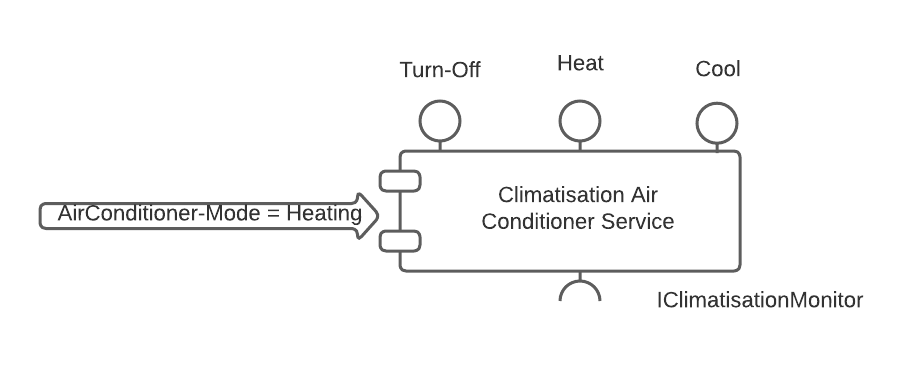
\includegraphics[scale=0.75]{cap_caso-estudio/images/adaption-loop-rule-heat} \\
    \hline

    \textbf{Regla:} & \emph{DisableAirConditionerWhenHeatingModeEnabledAndTargetTemperatureAchieved}  \\
    \textbf{Descripción:} & Apaga el aire acondicionado cuando el modo calefacción está activo y se ha alcanzado la temperatura de confort.  \\
    \textbf{Condición:} & \emph{airconditioner-mode} == \emph{Heating} \textbf{AND} \emph{temperature} >= \emph{target-temperature}  \\
    \textbf{Cuerpo:} &  \\
    & 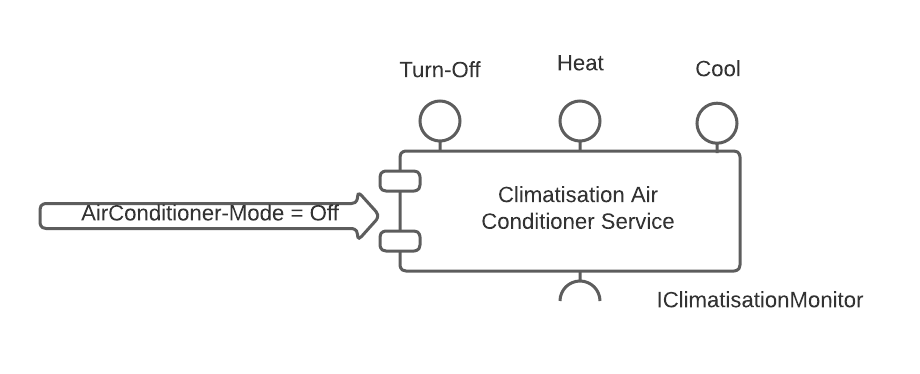
\includegraphics[scale=0.75]{cap_caso-estudio/images/adaption-loop-rule-off} \\
    \hline

    \textbf{Regla:} & \emph{EnableAirConditionerCoolingModeWhenTemperatureThresholdExceeded}  \\
    \textbf{Descripción:} & Activa el aire acondicionado en modo enfriar cuando la temperatura sea superior al umbral de calor.  \\
    \textbf{Condición:} & \emph{airconditioner-mode} != \emph{Cooling} \textbf{AND} \emph{temperature} >= \emph{hot-temperature-threshold}  \\
    \textbf{Cuerpo:} &  \\
    & 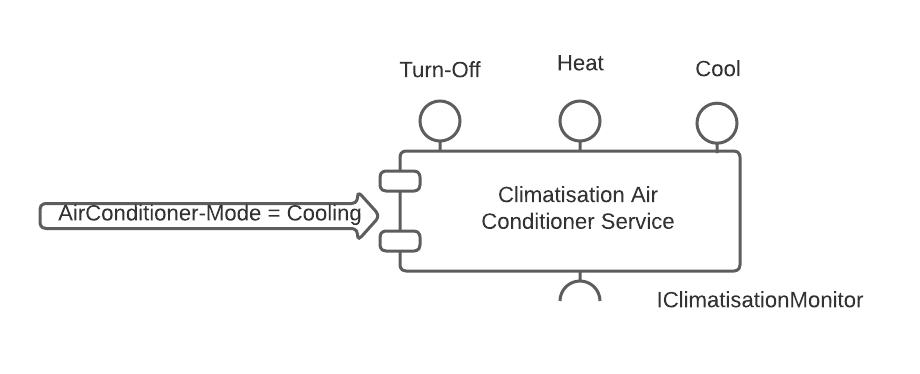
\includegraphics[scale=0.75]{cap_caso-estudio/images/adaption-loop-rule-cooling} \\
    \hline

    \textbf{Regla:} & \emph{DisableAirConditionerWhenCoolingModeEnabledAndTargetTemperatureAchieved}  \\
    \textbf{Descripción:} & Apaga el aire acondicionado cuando el modo enfiar está activo y se ha alcanzado la temperatura de confort.  \\
    \textbf{Condición:} & \emph{airconditioner-mode} == \emph{Cooling} \textbf{AND} \emph{temperature} <= \emph{target-temperature}  \\
    \textbf{Cuerpo:} &  \\
    & 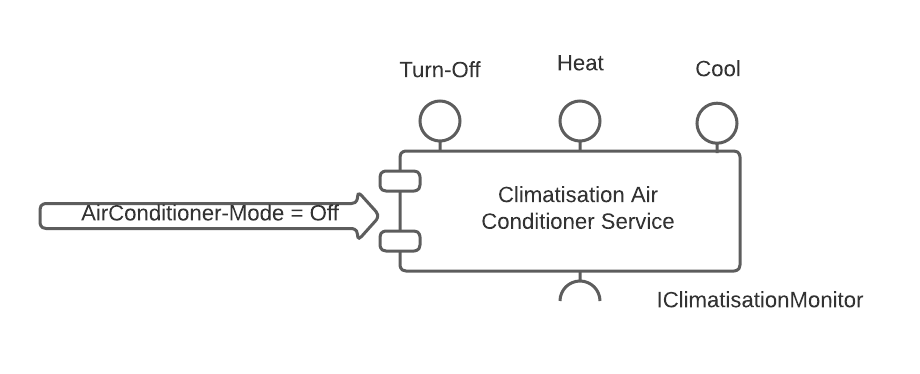
\includegraphics[scale=0.75]{cap_caso-estudio/images/adaption-loop-rule-off} \\
    \hline

  \caption{Reglas de adaptación del sistema de climatización.}
  \label{tab:adaption-rules-climatisation}
\end{longtable}

\subsection{Efectores:}

Una vez se evaluén estas reglas, solicitamos un cambio en la configuración del sistema. El módulo de planificación comprobará contra el conocimiento y el estado actual del sistema cuáles de los cambios solicitados es necesario aplicar. Si por ejemplo la propiedad ya tiene el valor solicitado, no hará falta ejecutarla.

El modulo de ejecución recibirá la petición y se la redirigirá a los efectores del sistema de climatización. En este caso, requerimos de efectores que cambien el modo del aire acondicionado según corresponda.

\begin{table}[htb]
  \centering

  \begin{tabular}{|r p{11.5cm}|}
    \hline
    \textbf{Efector:} & \emph{airconditioner.heat}  \\
    \textbf{Descripción:} & Activa el modo calentar del aire acondicionado. \\
    \hline
    \textbf{Efector:} & \emph{airconditioner.cool}  \\
    \textbf{Descripción:} & Activa el modo enfriar del aire acondicionado. \\
    \hline
    \textbf{Efector:} & \emph{airconditioner.turn-off}  \\
    \textbf{Descripción:} & Apaga el aire acondicionado. \\
    \hline
  \end{tabular}

  \caption{Efectores del sistema de climatización.}
    \label{tab:climatisation-effectors}
\end{table}

Hecho esto, el sistema se adapta a a la nueva situación, y reportará una nueva temperatura en cuanto corresponda. La temperatura variará dependiendo de si está apagado o no.

\subsection{Configuración del sistema}

Requerimos entonces 4 servicios para implementar la solución: Servicio de aire acondicionado, monitor de climatización, el servicio de reglas y el servicio de efectores. Con ellos, podemos adaptarnos al bucle MAPE-K descrito en el capítulo %TODO: Capítulo.

\section{Implementación}

Para la implementación, hemos utilizado las mismas tecnologías que en los servicios del bucle MAPE-K: microservicios en ASP.NET Core, empaquetados en contenedores de Docker para facilitar su despliegue. Generamos los API Clients con OpenAPI y demás.

Como no disponemos de un aire acondicionado real, hemos optado por implementar uno ficticio. Cuando está apagado, la temperatura aumenta o disminuye según una configuración del fake. De esta forma, podemos simular los cambios de temperatura más rápido y ver si se aplican las adaptaciones pertinentes.

\subsection{Telemetría}

Un punto en el que queremos hacer hincapié es en la telemetría. Debido a que estamos tratando con un sistema distribuido es complicado conocer el estado del sistema en determinado momento. Especialmente en este caso, que participan más de diez servicios distintos.

Por defecto, solo contábamos con los \emph{logs} de consola, que mostramos en la figura \ref{fig:console-logs}. Aparecen en una única ventana intercalados los registros de todos los servicios. Aunque nos pueden resultar útil, es una aproximación ineficiente y según aumente la escala de peticiones simultáneamente se volverá más difícil de interpretar.

\begin{figure}[h]
  \centering
  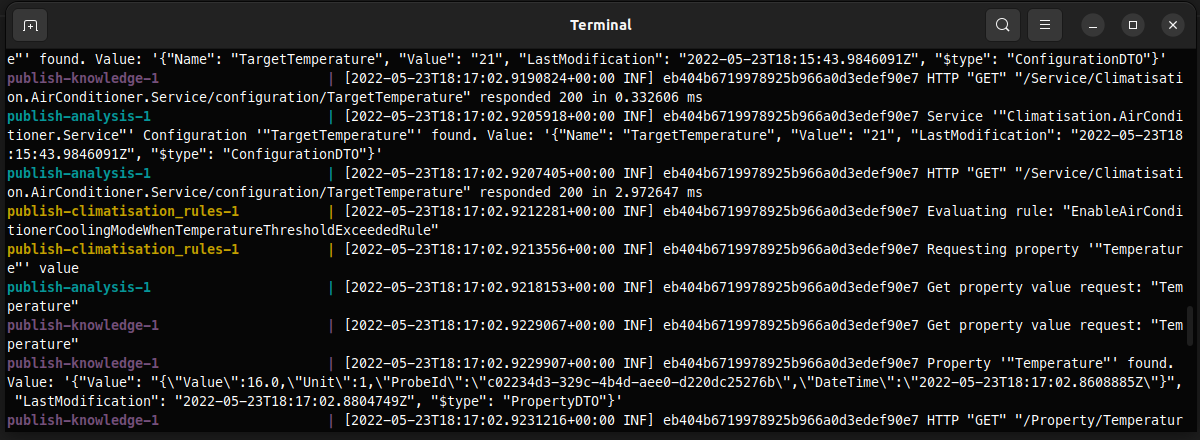
\includegraphics[scale=1.45]{cap_caso-estudio/images/console-logs}
  \caption{Extracto de \emph{logs} de una ejecución habitual.}
  \label{fig:console-logs}
\end{figure}

Por ello, para que resultara más sencillo trabajar en la implementación de los servicios y diagnosticar qué ocurre con el sistema, decidimos implementar una solución de observabilidad. La observabilidad es \cite{parkerProblemDistributedTracing2020} y consta de tres partes distintas: %TODO CITA
\begin{itemize}
  \item \textbf{Logs}: \textcolor{red}{A recording of an Event. Typically the record includes a timestamp indicating when the Event happened as well as other data that describes what happened, where it happened, etc. \cite{opentelemetryOpenTelemetryDocumentation2022} Provide extremely fine-grained detail on a given service, but have no built-in way to provide that detail in the context of a request. \cite{parkerProblemDistributedTracing2020}}
  \item \textbf{Métricas}: \textcolor{red}{Son agregados que nos permiten conocer el estado de las estancias de nuestros servicios. Records a data point, either raw measurements or predefined aggregation, as timeseries with Metadata. \cite{opentelemetryOpenTelemetryDocumentation2022}}
  \item \textbf{Trazas distribuidas}: \textcolor{red}{Tracks the progression of a single Request, called a Trace, as it is handled by Services that make up an Application. A Distributed Trace transverses process, network and security boundaries. \cite{opentelemetryOpenTelemetryDocumentation2022}  providing visibility into the operation of your microservice architecture. It allows you to gain critical insights into the performance and status of individual services as part of a chain of requests in a way that would be difficult or time-consuming to do otherwise. Distributed tracing gives you the ability to understand exactly what a particular, individual service is doing as part of the whole, enabling you to ask and answer questions about the performance of your services and your distributed system. \cite{parkerProblemDistributedTracing2020}}
\end{itemize}

Para poder capturar todos estos elementos, optamos por usar el estándar OpenTelemetry. Se trata de una librería estándar utilizada para instrumentar el código de las aplicaciones. Distintas compañías del ámbito de la telemetría software ofrecen APIs que capturan el output de esta librería.

Gracias a él pudimos capturar la telemetría de la siguiente forma implementar usando tres servicios distintos:

\begin{figure}[h]
  \centering
  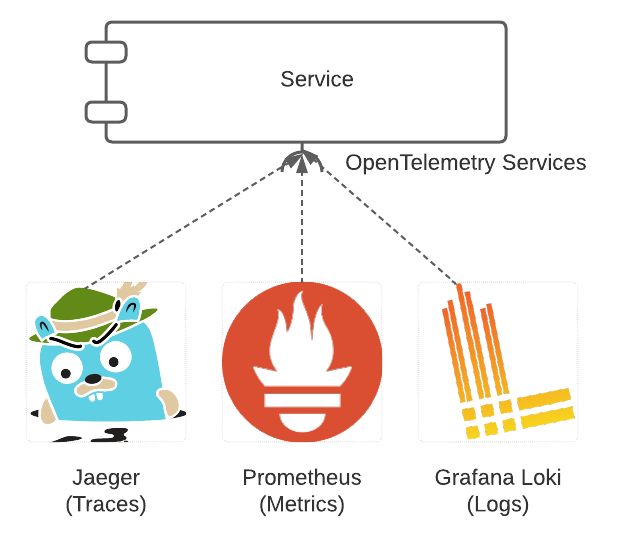
\includegraphics[scale=0.75]{cap_caso-estudio/images/observability-telemetry-collection}
  \caption{Extracto de \emph{logs} de una ejecución habitual.}
  \label{fig:observability-telemetry-collection}
\end{figure}

\subsubsection{Loki: Logs}
Lo primero que queremos ver es cómo mejorar nuestra estrategia de logging. Lo ideal es añadir identificadores de correlación (el traceID), que nos permita rastrear a través de los distintos servicios una misma traza. Por ejemplo, podemos filtrar a partir de ella para ver todos los detalles de los servicios que intervinieron.

\subsubsection{Jaeger: Trazas distribuidas}

Gracias a las trazas distribuidas, podemos ver todas las actividades por las que pasó una petición. En nuestro caso, podemos ver por todos los estados por los que paso.

\subsubsection{Prometheus: Métricas}


\subsubsection{Grafana: Visualización}

Desarrollamos un panel de monitorización con Grafana. Esto nos permitía consultar en un solo lugar las métricas, los logs y las trazas.


%%%%%%%%%%%%%%%%%%%%%%%%%%%%%%%%%%%%%%%%%%%%%%%%%%%%%%%%%%%%%%%%%%%%%%%%%%%%%%%
%                                 CONCLUSIONS                                 %
%%%%%%%%%%%%%%%%%%%%%%%%%%%%%%%%%%%%%%%%%%%%%%%%%%%%%%%%%%%%%%%%%%%%%%%%%%%%%%%

\chapter{Conclusions}

????? ????????????? ????????????? ????????????? ????????????? ?????????????

%%%%%%%%%%%%%%%%%%%%%%%%%%%%%%%%%%%%%%%%%%%%%%%%%%%%%%%%%%%%%%%%%%%%%%%%%%%%%%%
%                                BIBLIOGRAFIA                                 %
%%%%%%%%%%%%%%%%%%%%%%%%%%%%%%%%%%%%%%%%%%%%%%%%%%%%%%%%%%%%%%%%%%%%%%%%%%%%%%%

\bibliography{bibliography}

\cleardoublepage

%%%%%%%%%%%%%%%%%%%%%%%%%%%%%%%%%%%%%%%%%%%%%%%%%%%%%%%%%%%%%%%%%%%%%%%%%%%%%%%
%                           APÈNDIXS  (Si n'hi ha!)                           %
%%%%%%%%%%%%%%%%%%%%%%%%%%%%%%%%%%%%%%%%%%%%%%%%%%%%%%%%%%%%%%%%%%%%%%%%%%%%%%%

\APPENDIX

%%%%%%%%%%%%%%%%%%%%%%%%%%%%%%%%%%%%%%%%%%%%%%%%%%%%%%%%%%%%%%%%%%%%%%%%%%%%%%%
%                         LA CONFIGURACIO DEL SISTEMA                         %
%%%%%%%%%%%%%%%%%%%%%%%%%%%%%%%%%%%%%%%%%%%%%%%%%%%%%%%%%%%%%%%%%%%%%%%%%%%%%%%

\chapter{Configuració del sistema}

????? ????????????? ????????????? ????????????? ????????????? ?????????????

\section{Fase d'inicialització}

????? ????????????? ????????????? ????????????? ????????????? ?????????????

\section{Identificació de dispositius}

????? ????????????? ????????????? ????????????? ????????????? ?????????????

%%%%%%%%%%%%%%%%%%%%%%%%%%%%%%%%%%%%%%%%%%%%%%%%%%%%%%%%%%%%%%%%%%%%%%%%%%%%%%%
%                               ALTRES  APÈNDIXS                              %
%%%%%%%%%%%%%%%%%%%%%%%%%%%%%%%%%%%%%%%%%%%%%%%%%%%%%%%%%%%%%%%%%%%%%%%%%%%%%%%


\chapter{??? ???????????? ????}

????? ????????????? ????????????? ????????????? ????????????? ?????????????



%%%%%%%%%%%%%%%%%%%%%%%%%%%%%%%%%%%%%%%%%%%%%%%%%%%%%%%%%%%%%%%%%%%%%%%%%%%%%%%
%                              FI DEL DOCUMENT                                %
%%%%%%%%%%%%%%%%%%%%%%%%%%%%%%%%%%%%%%%%%%%%%%%%%%%%%%%%%%%%%%%%%%%%%%%%%%%%%%%

\end{document}
